% Explication des étapes de l'alogorithme par un exemple d'Evaluation:

\subsection{Case study}
\label{sec:case_study}

In this section we demonstrate how this method generates a PH model coherent with the set of biological regulatory time series data given as an input. 
First, the method uses discritised observations as an input (\ie chronogram), thus it is necessary to use an other method which transforms the analogic time series data to discritised time series data.

%\begin{figure}[htb!]
%Observations:\\
%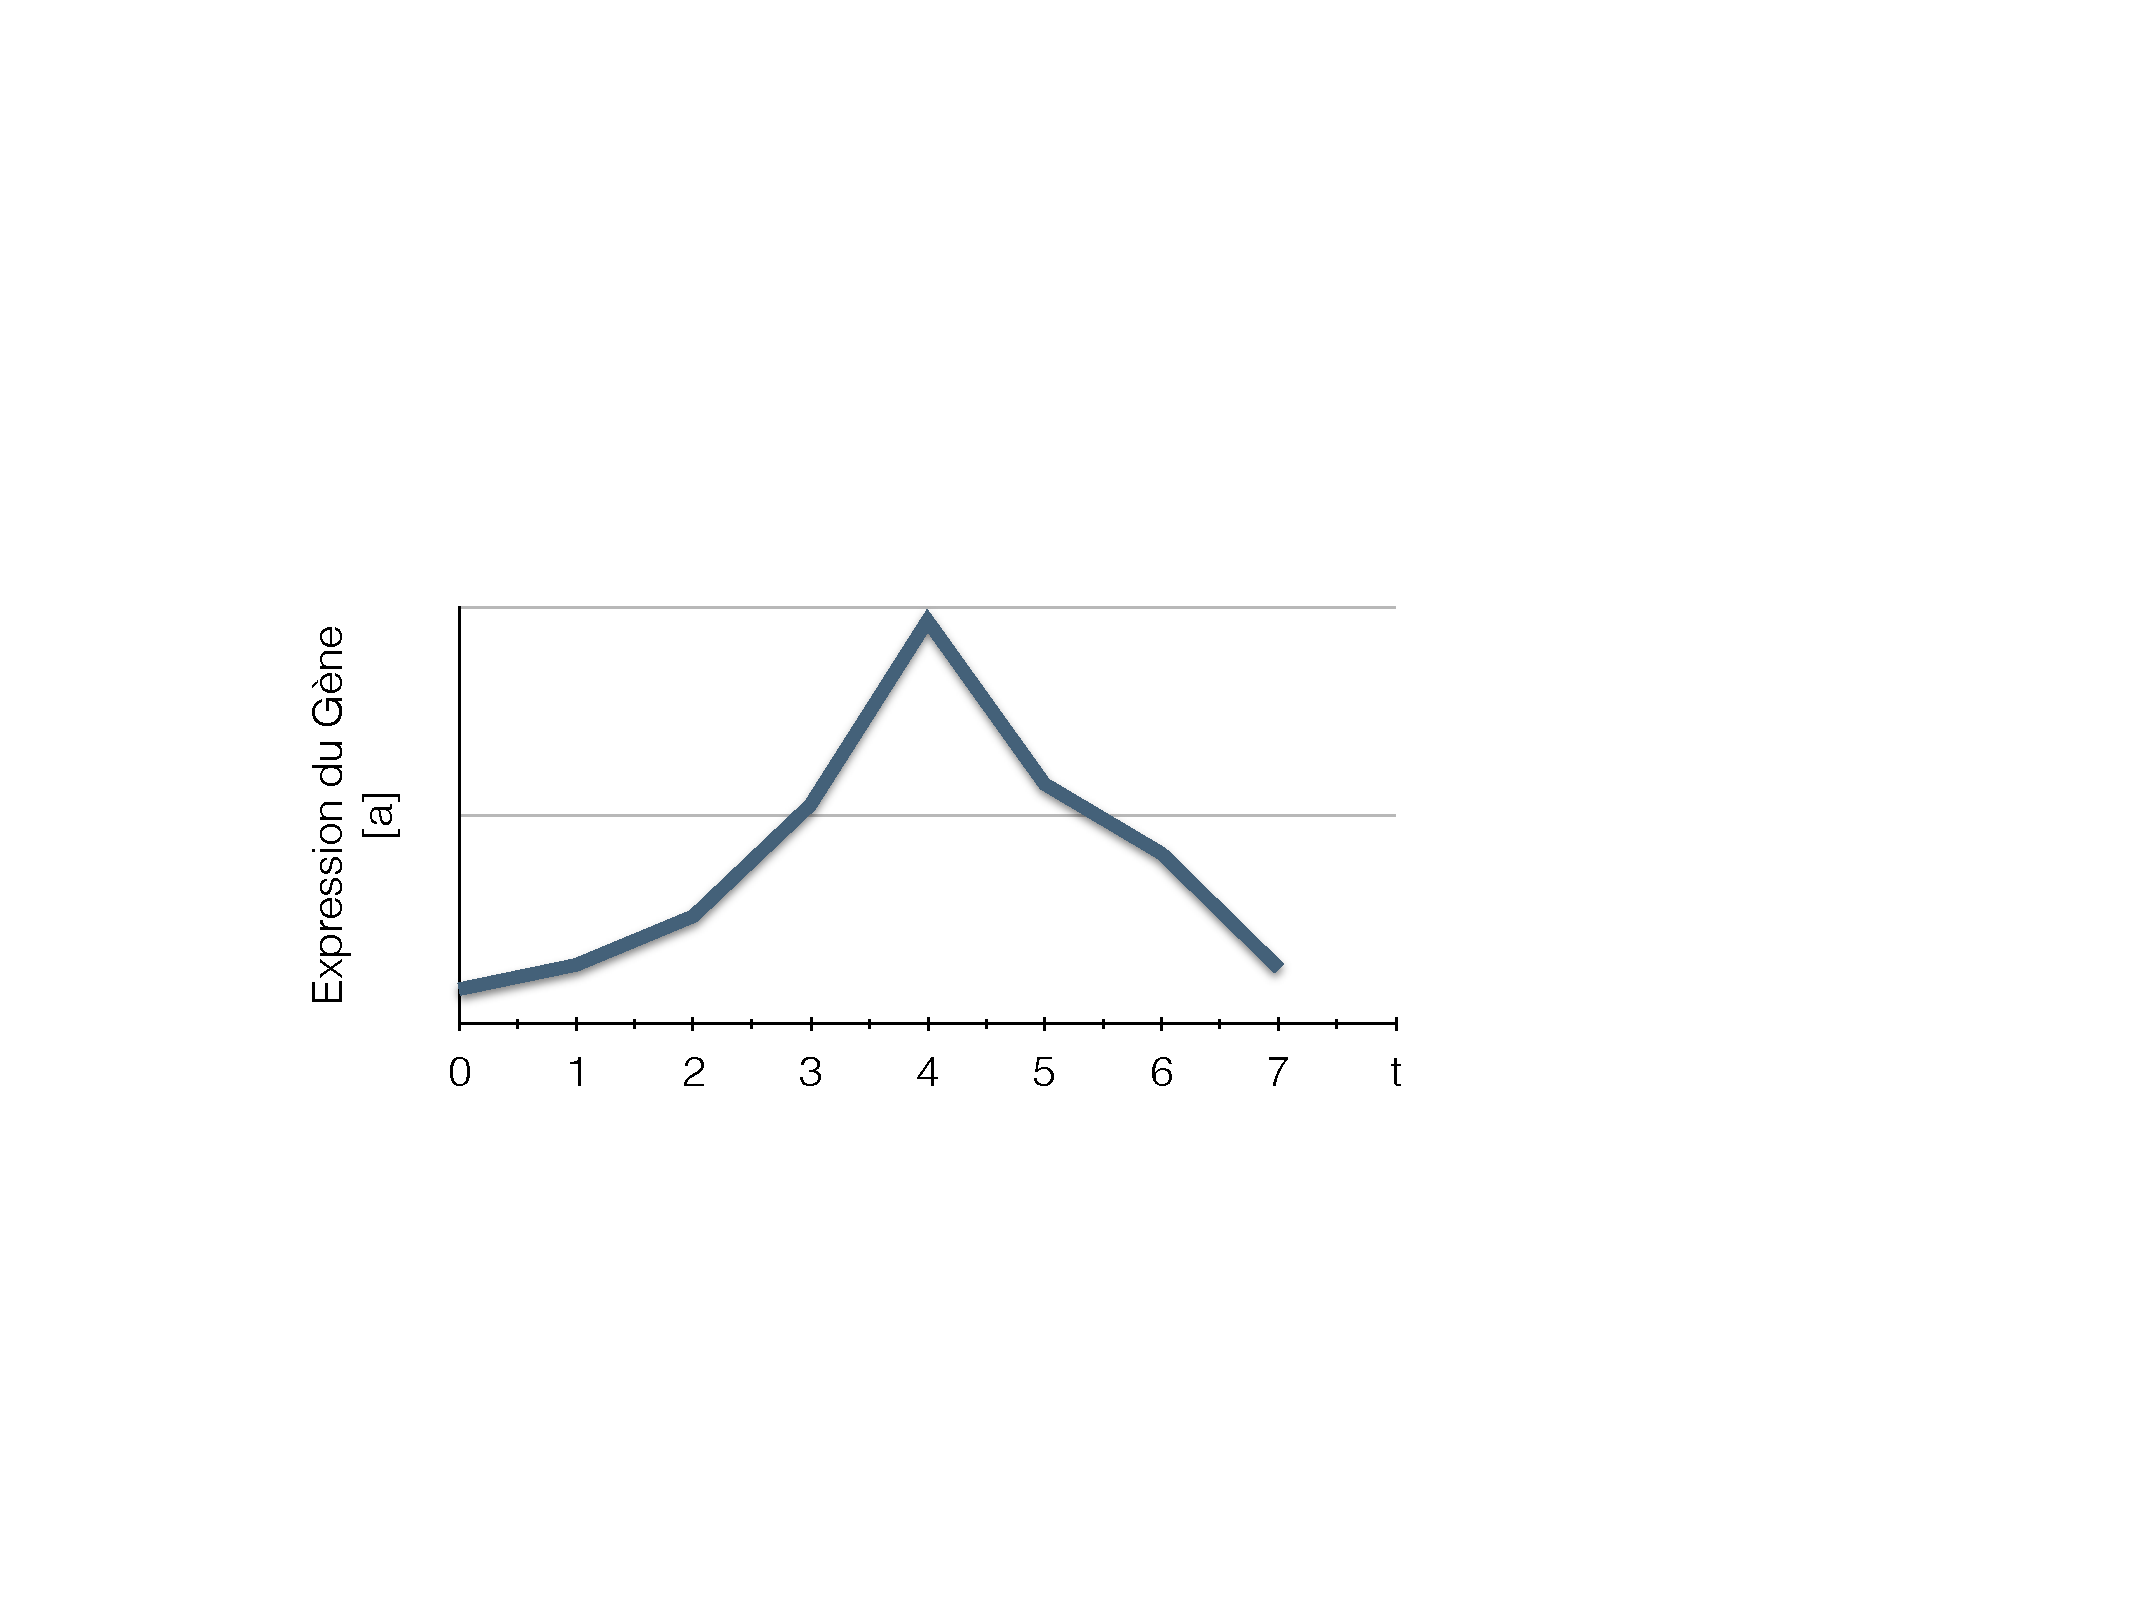
\includegraphics[ width =0.35\linewidth]{images/courbes/gene-a.pdf}\\
%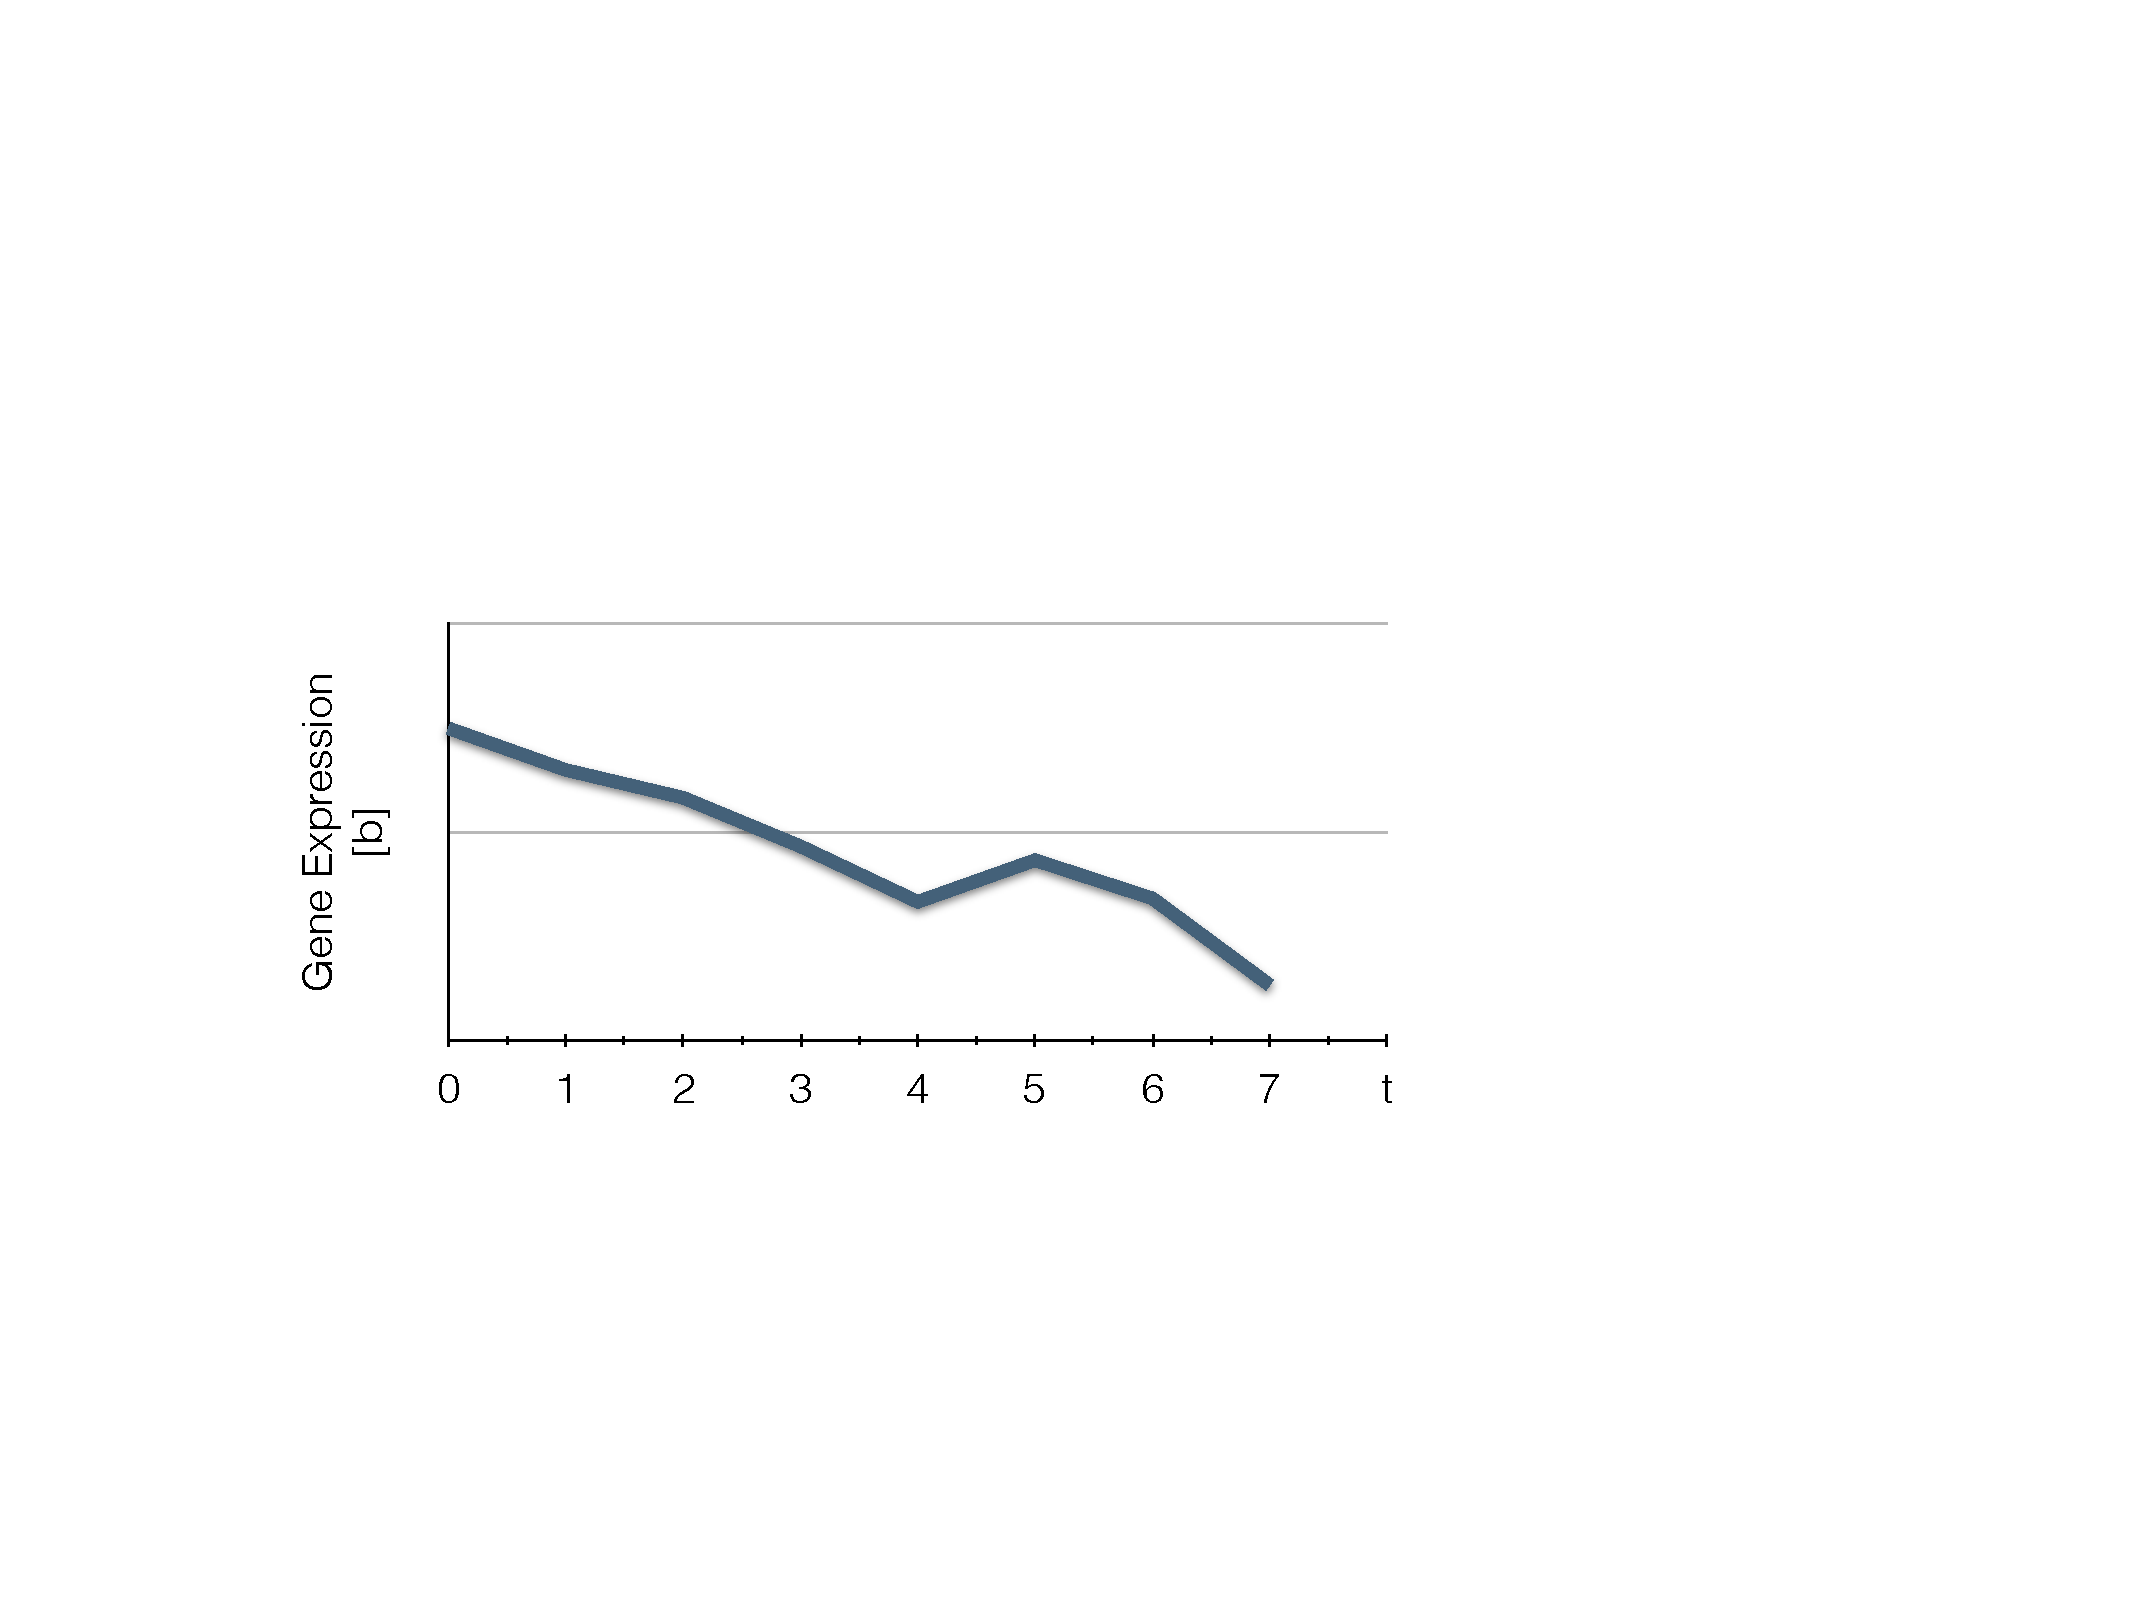
\includegraphics[ width =0.35\linewidth]{images/courbes/gene-b.pdf}\\
%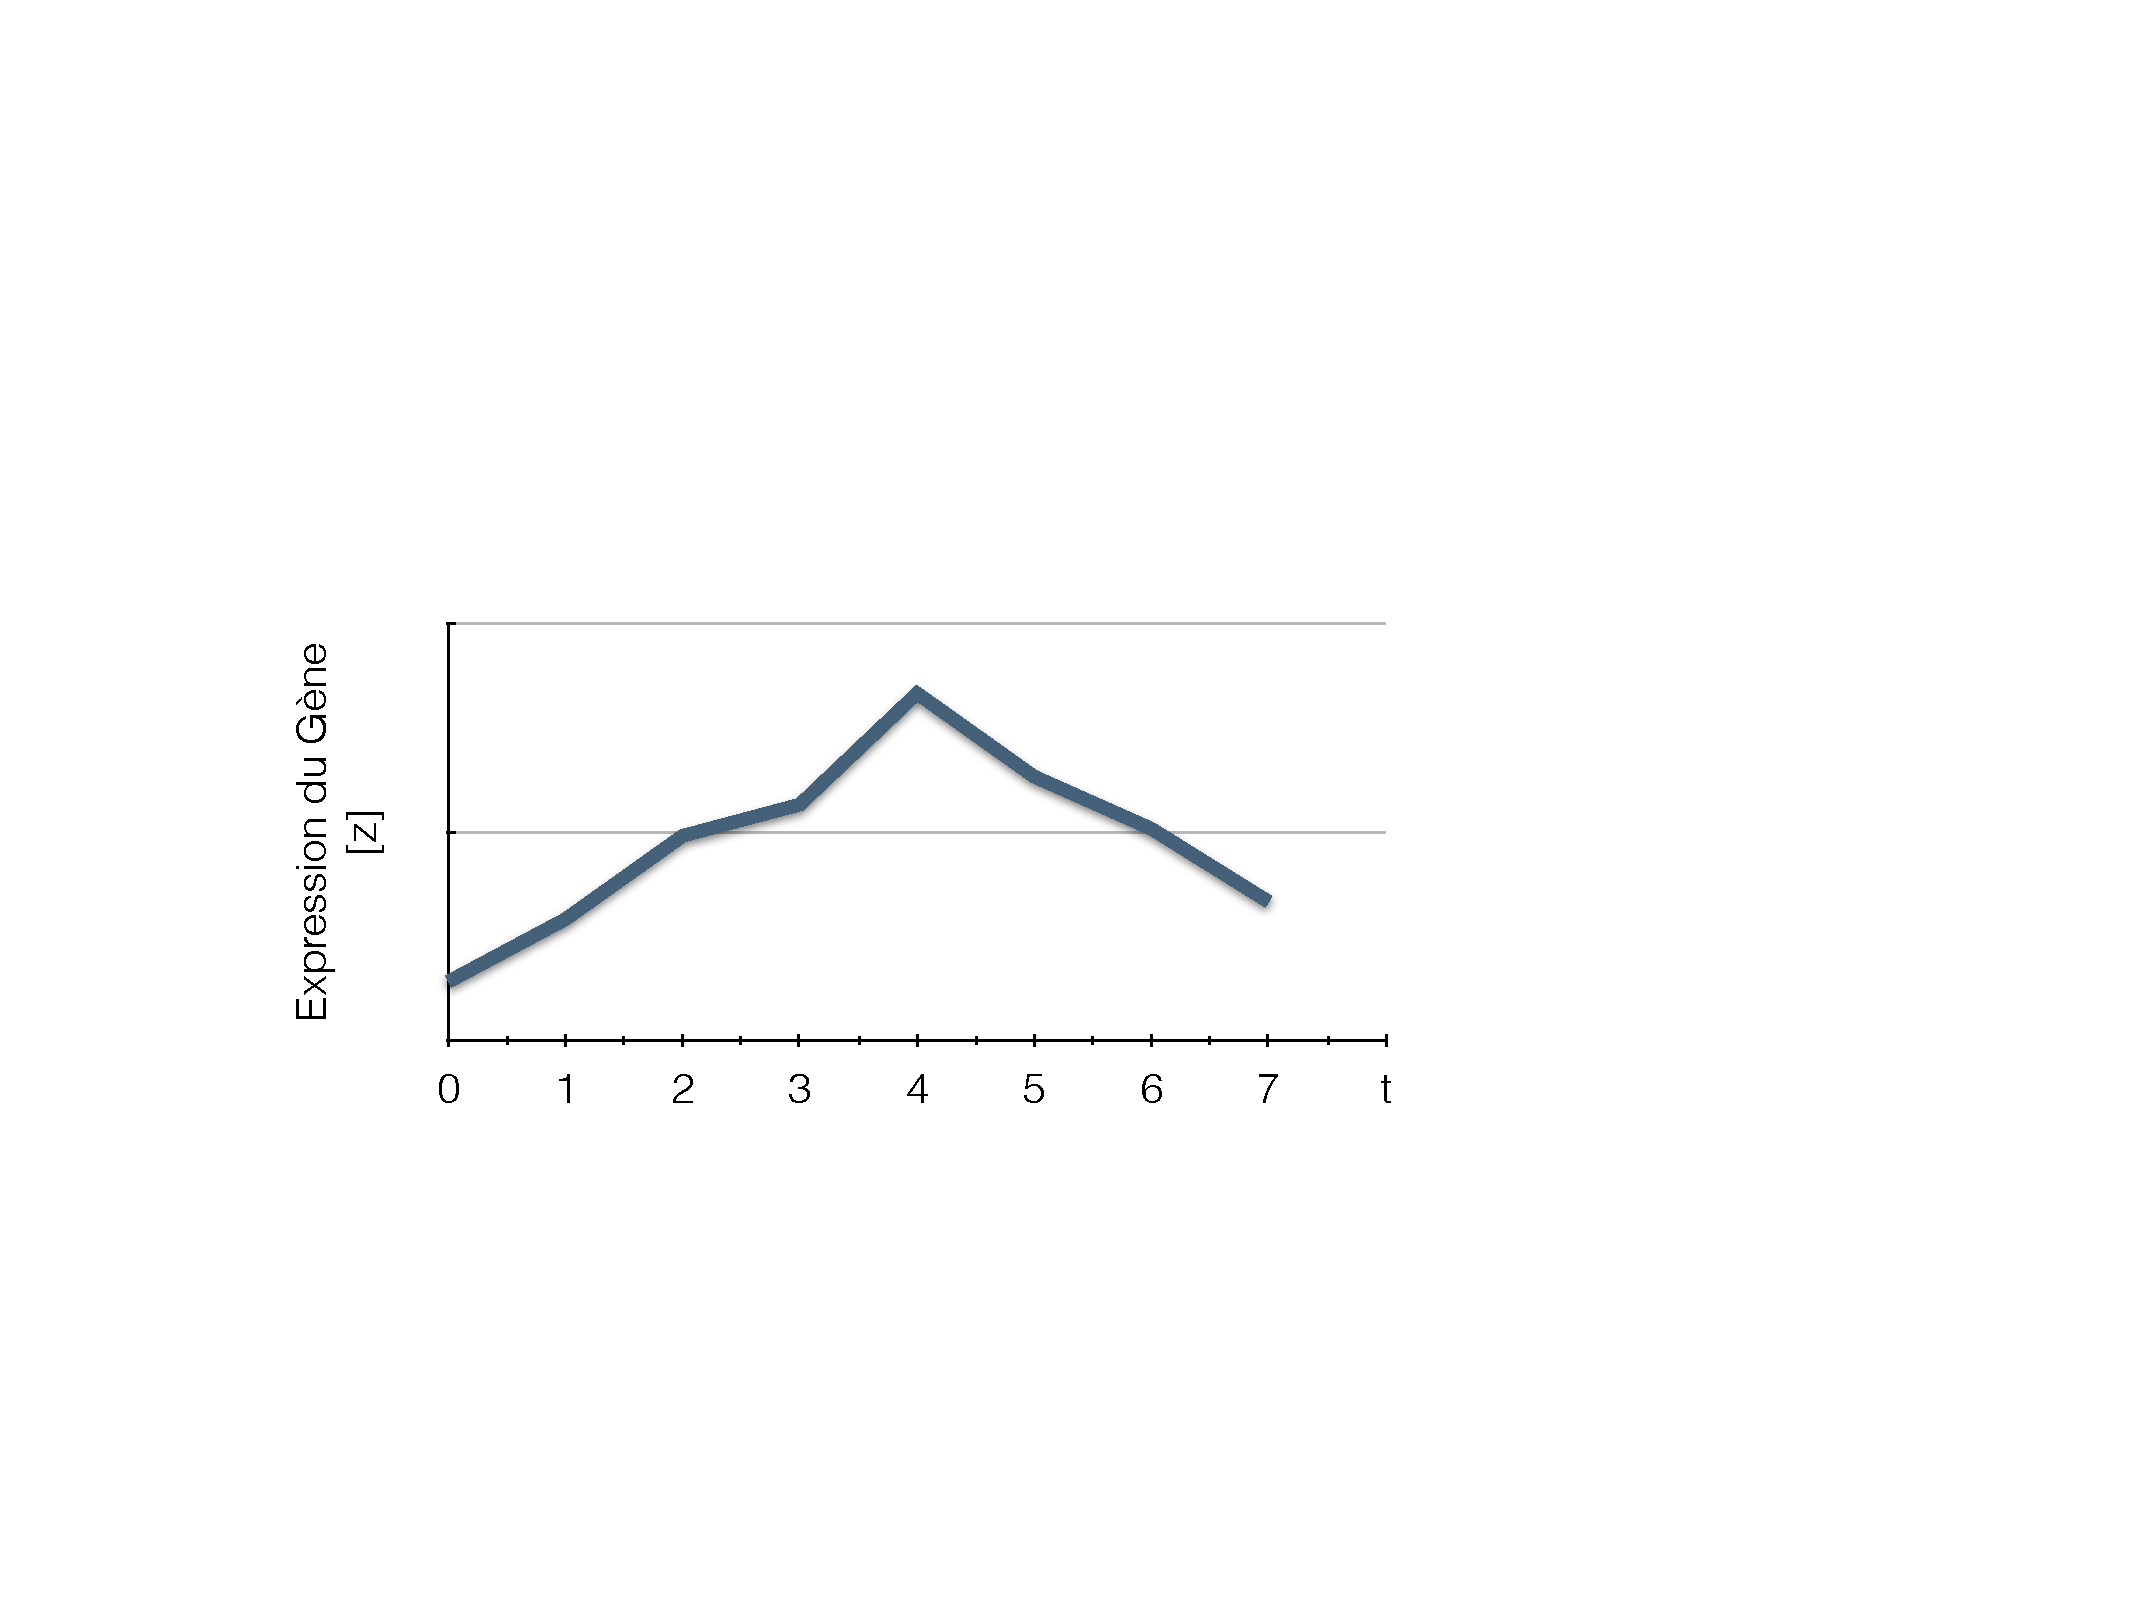
\includegraphics[ width =0.35\linewidth]{images/courbes/gene-z.pdf}
%\hspace{0.01cm}
%\textcolor{red}{$\Rightarrow$}
%\hspace{0.01cm}
%\begin{minipage}[t]{0.4\linewidth}
%\vspace{-5cm}
%Process Hitting:
%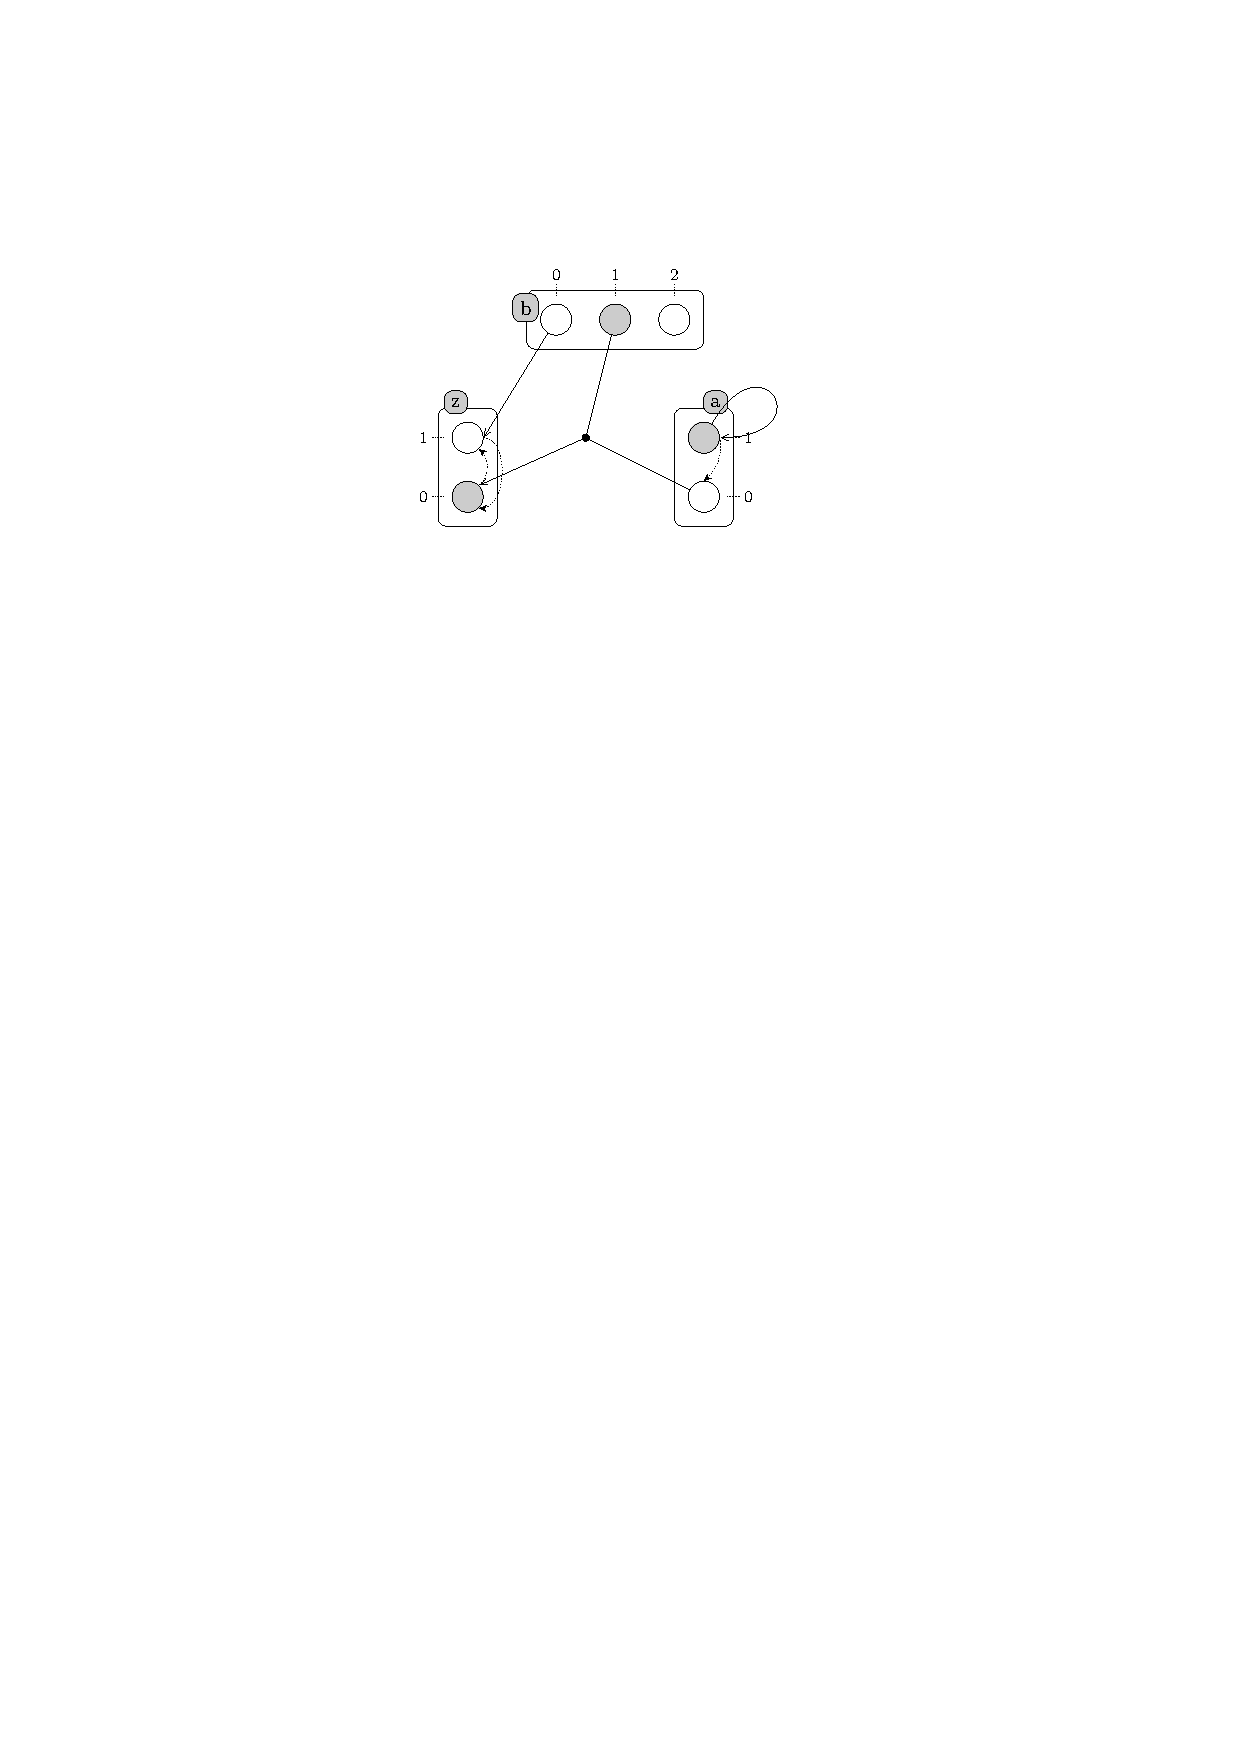
\includegraphics[width =1\linewidth]{images/PH-but.pdf}
%\end{minipage}
%\end{figure}


% Discretization figure
\begin{figure}[h]\centering
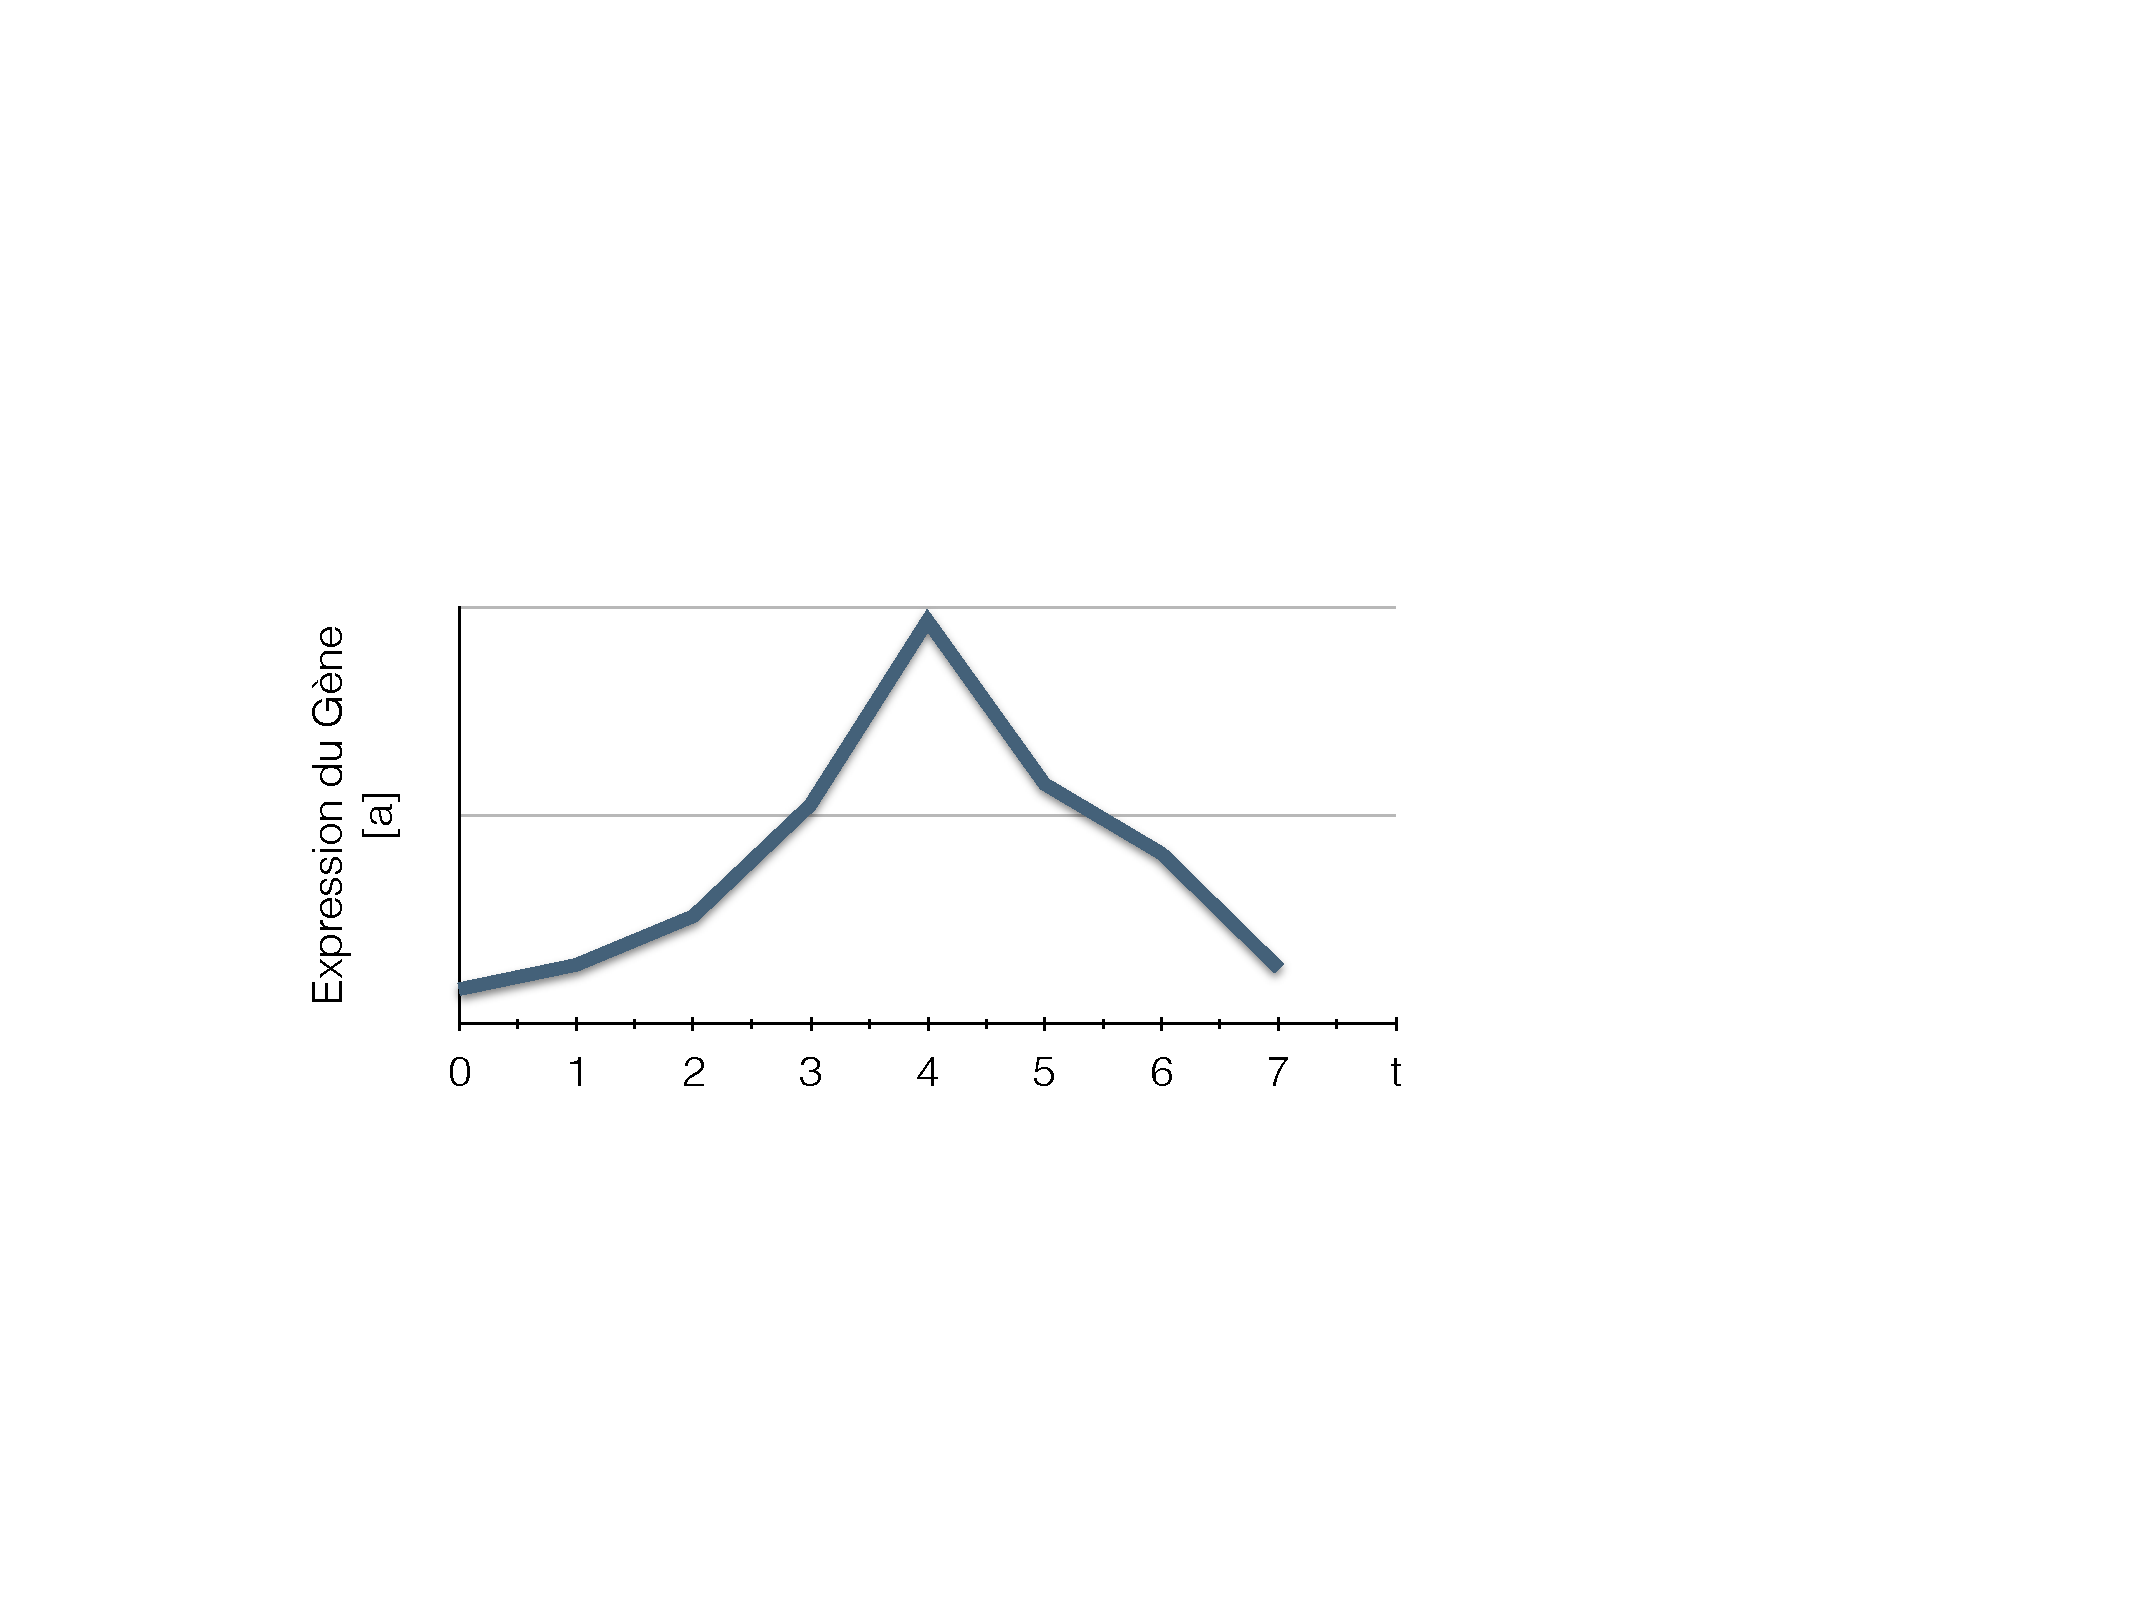
\includegraphics[width =0.31\linewidth]{images/courbes/gene-a.pdf}
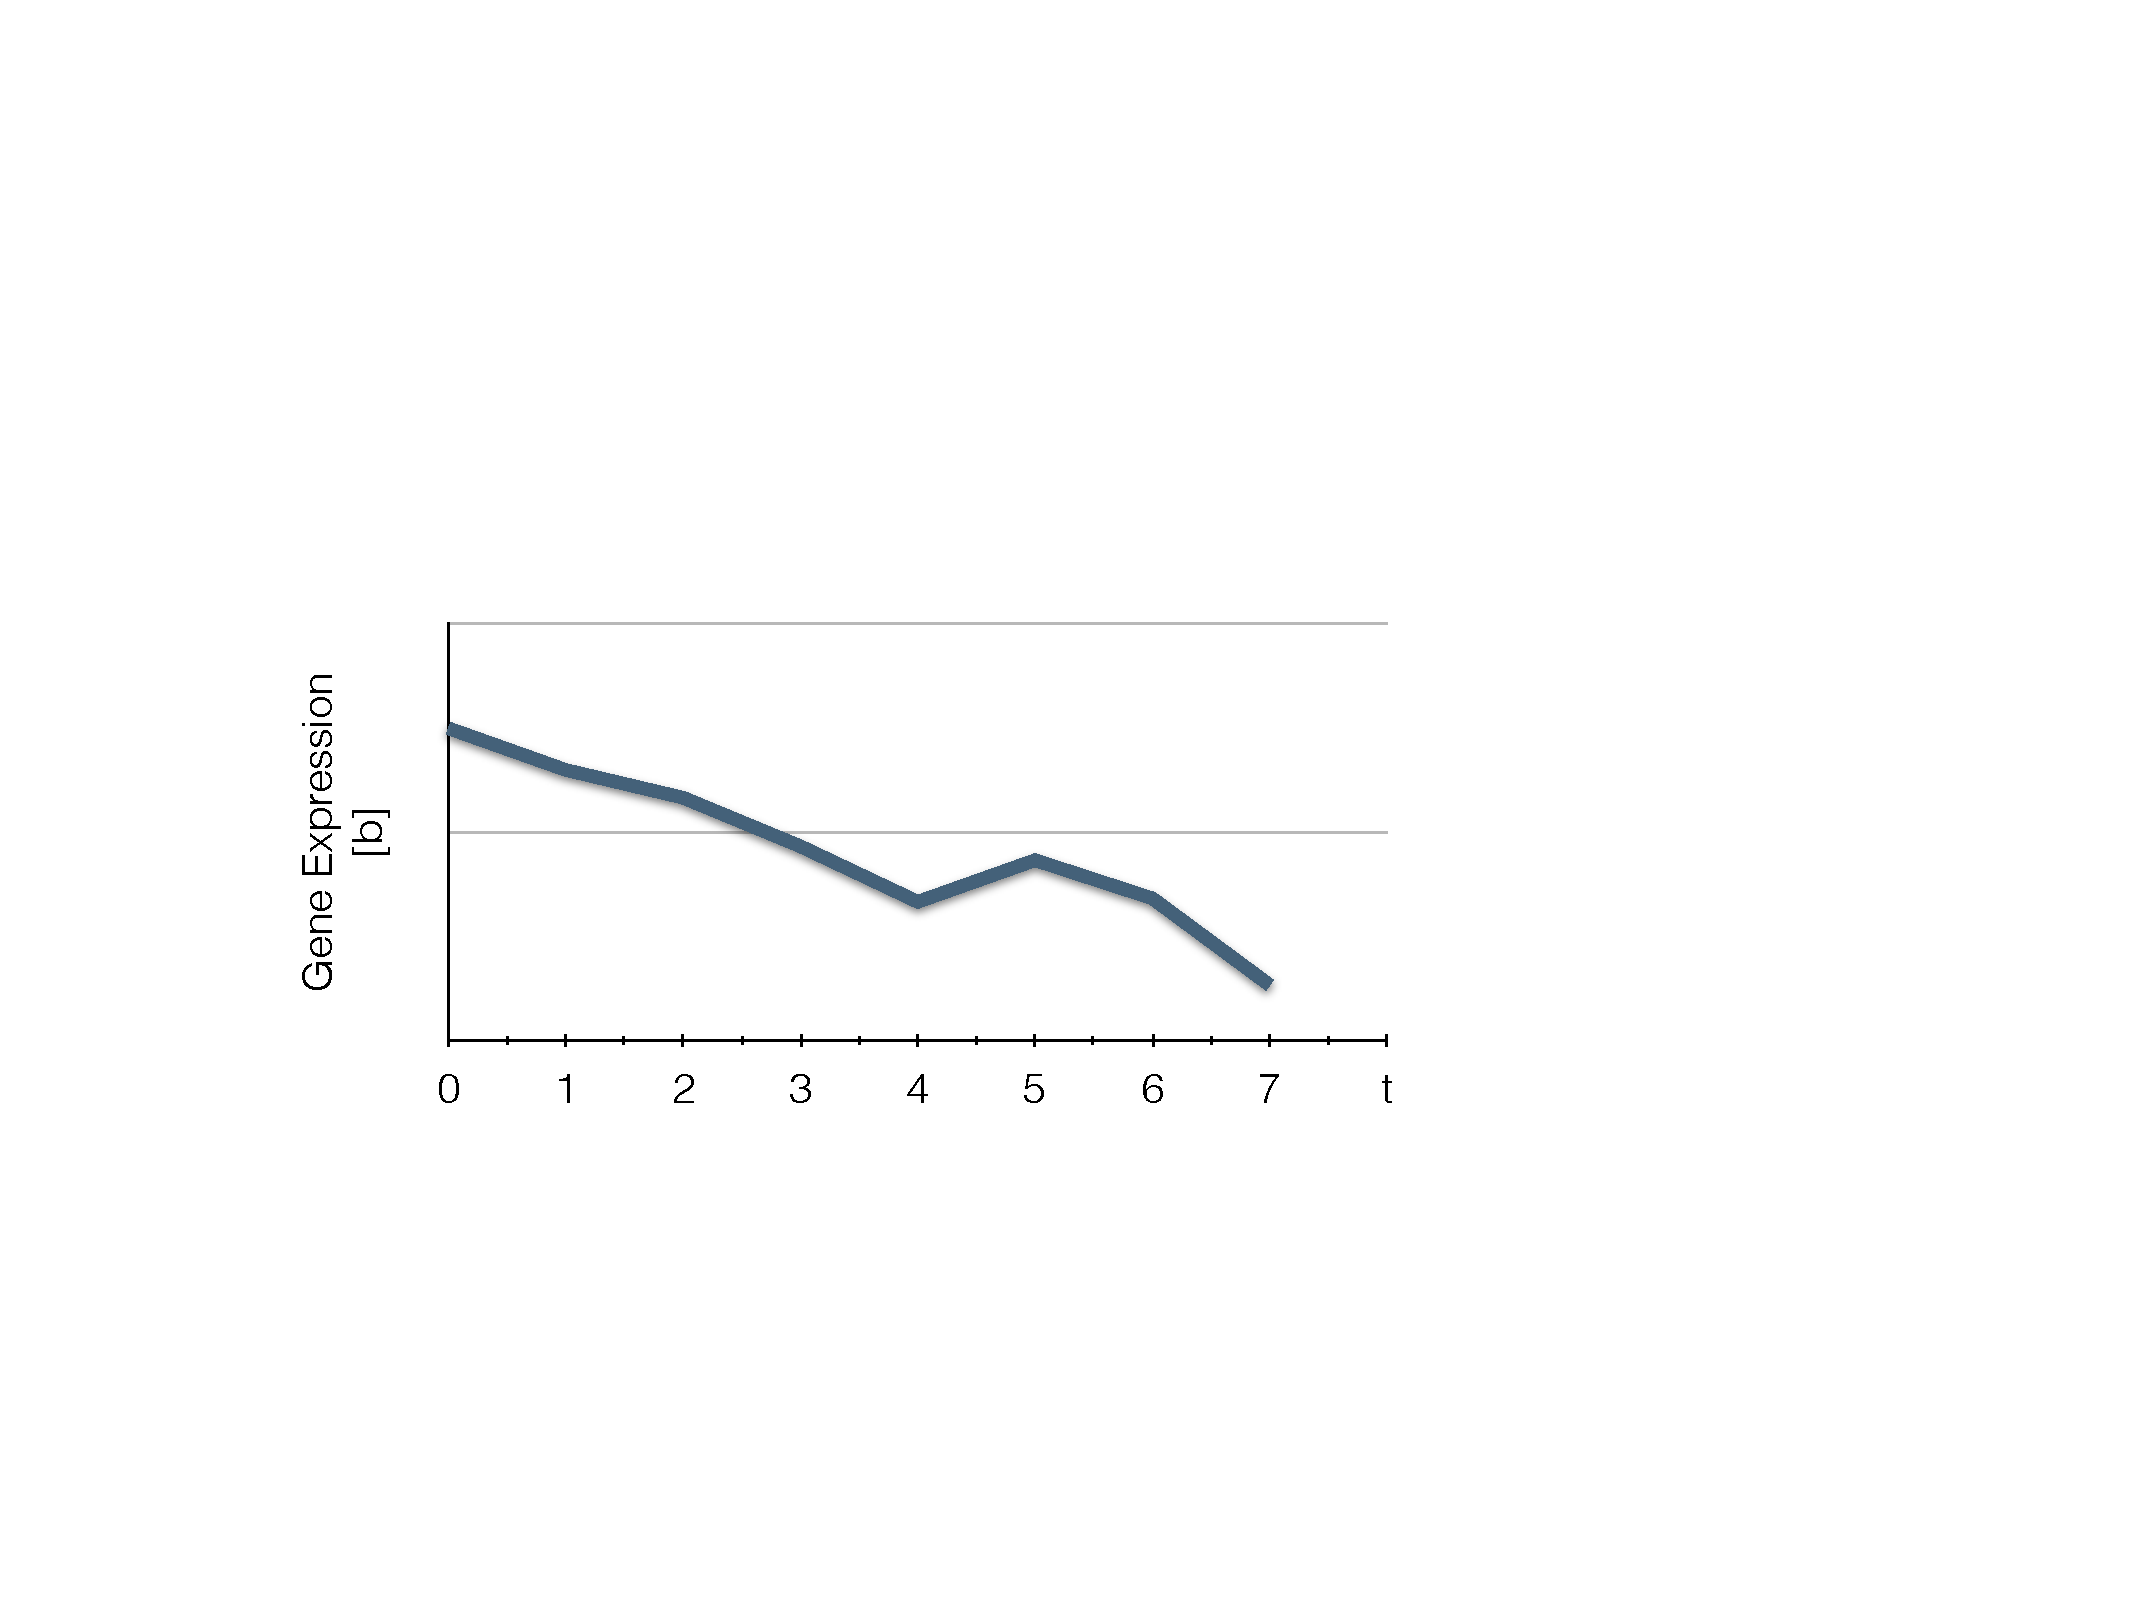
\includegraphics[width =0.31\linewidth]{images/courbes/gene-b.pdf}
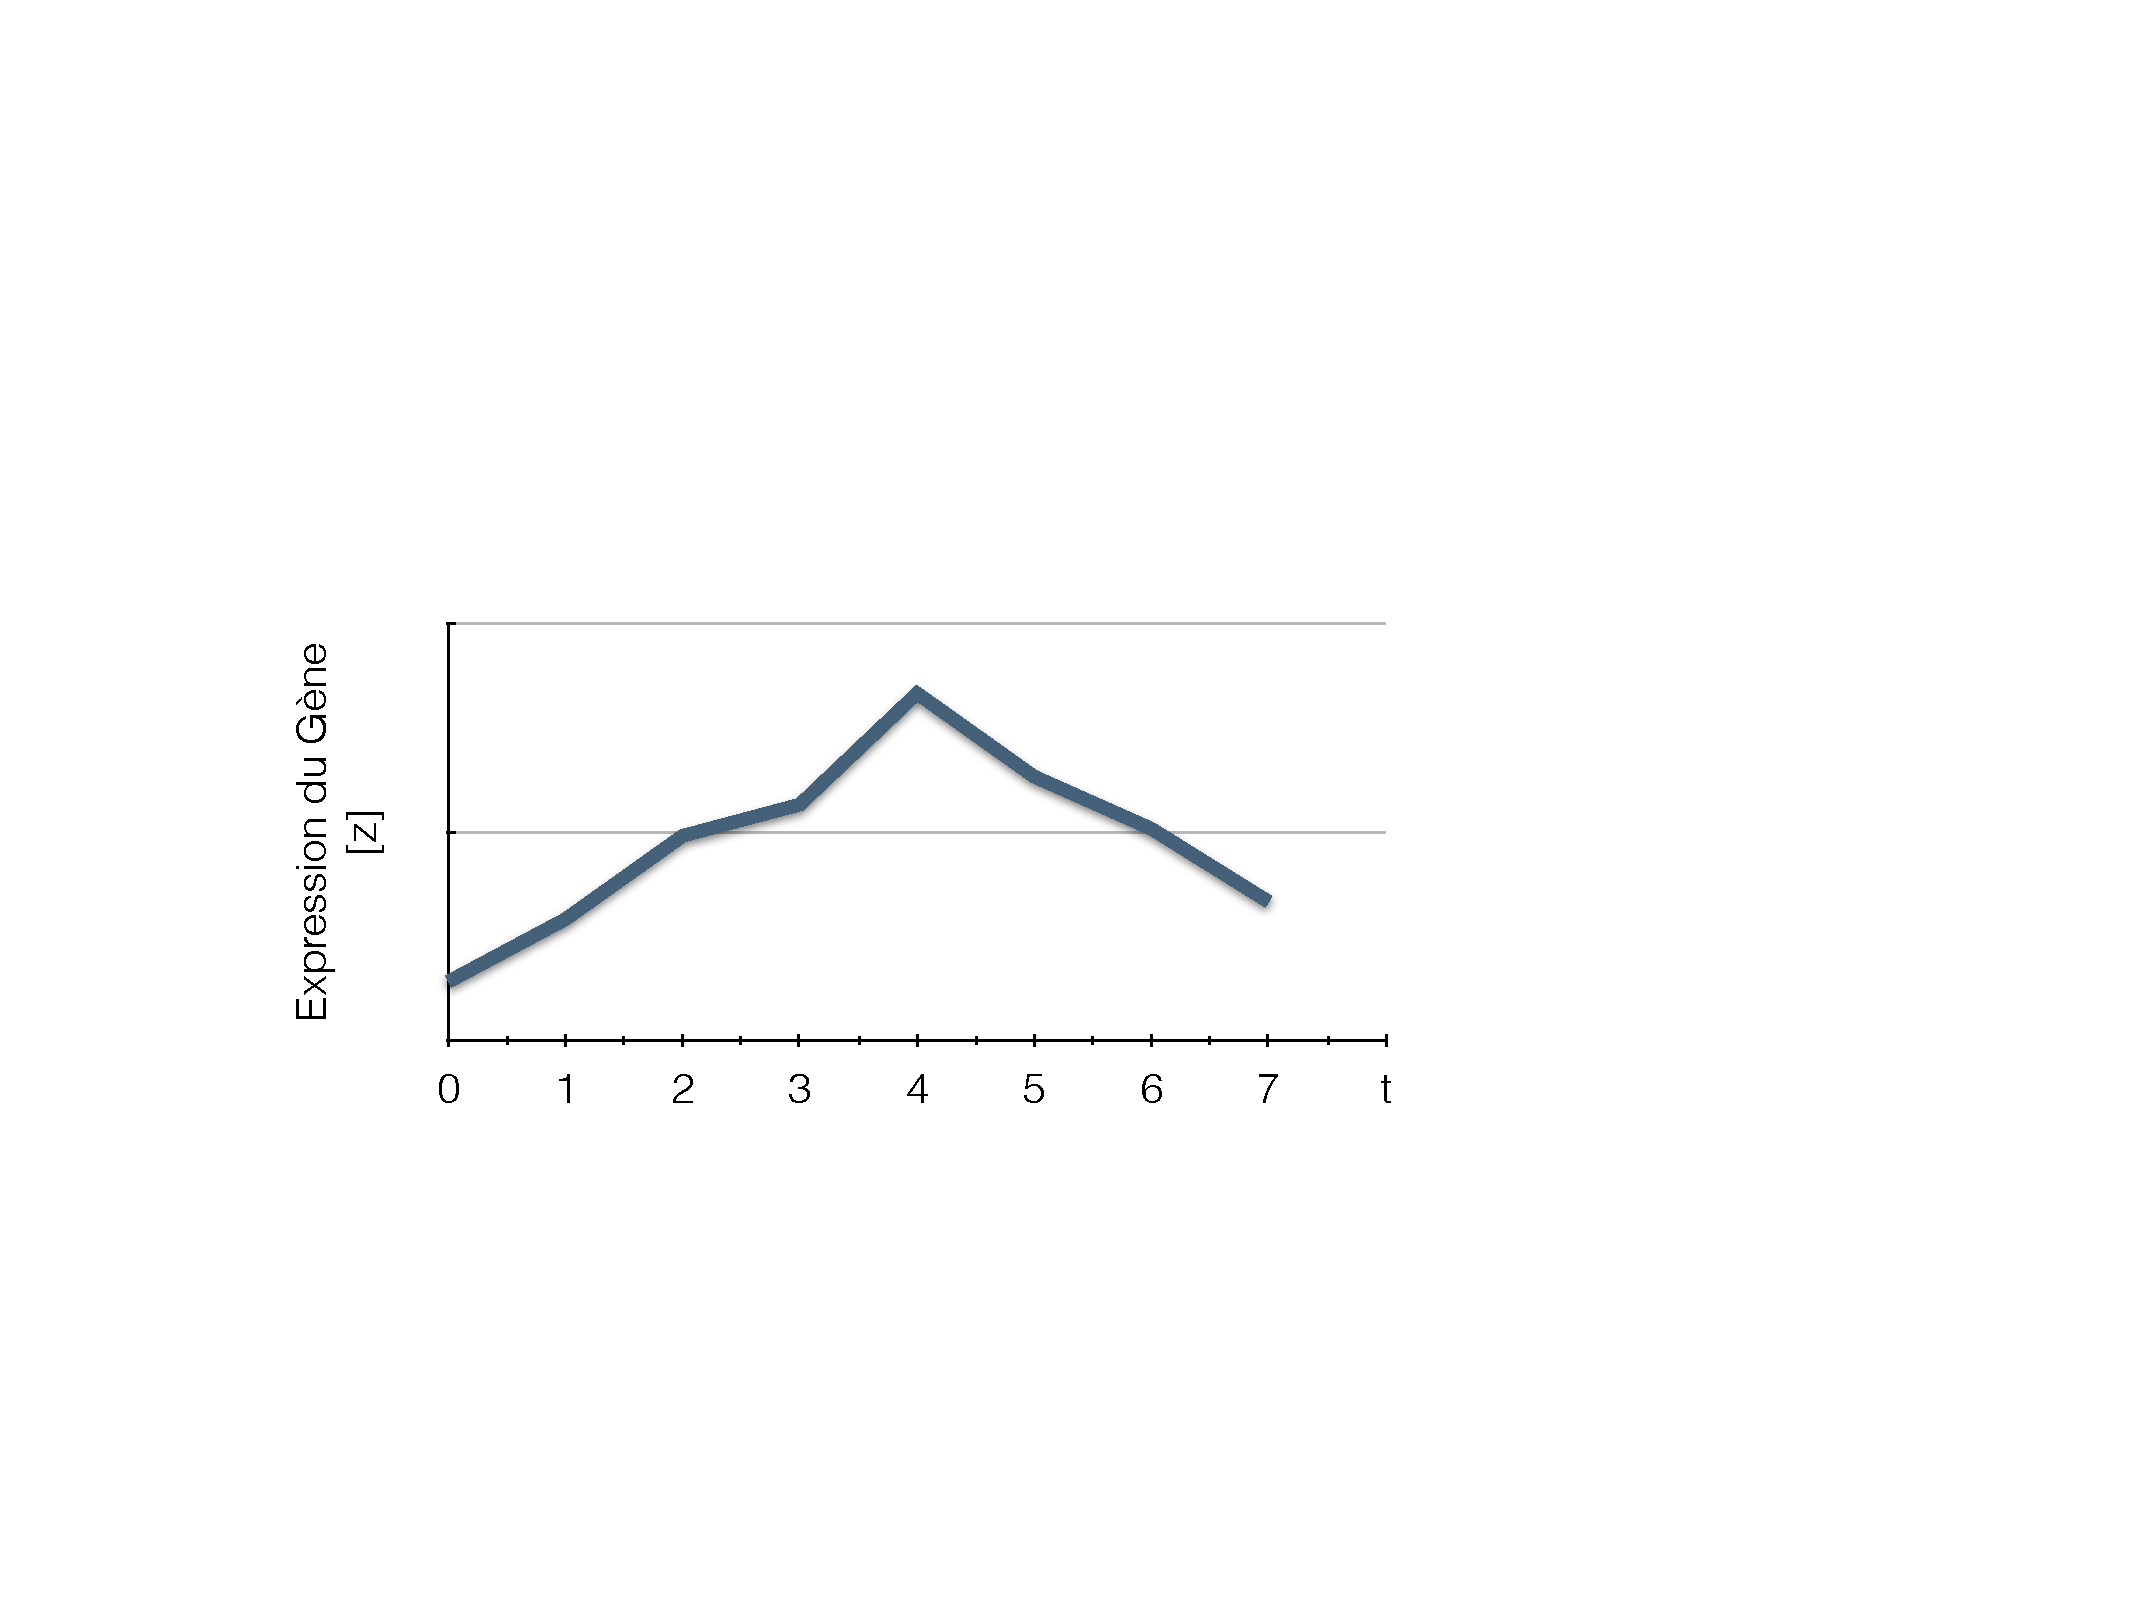
\includegraphics[width =0.31\linewidth]{images/courbes/gene-z.pdf}

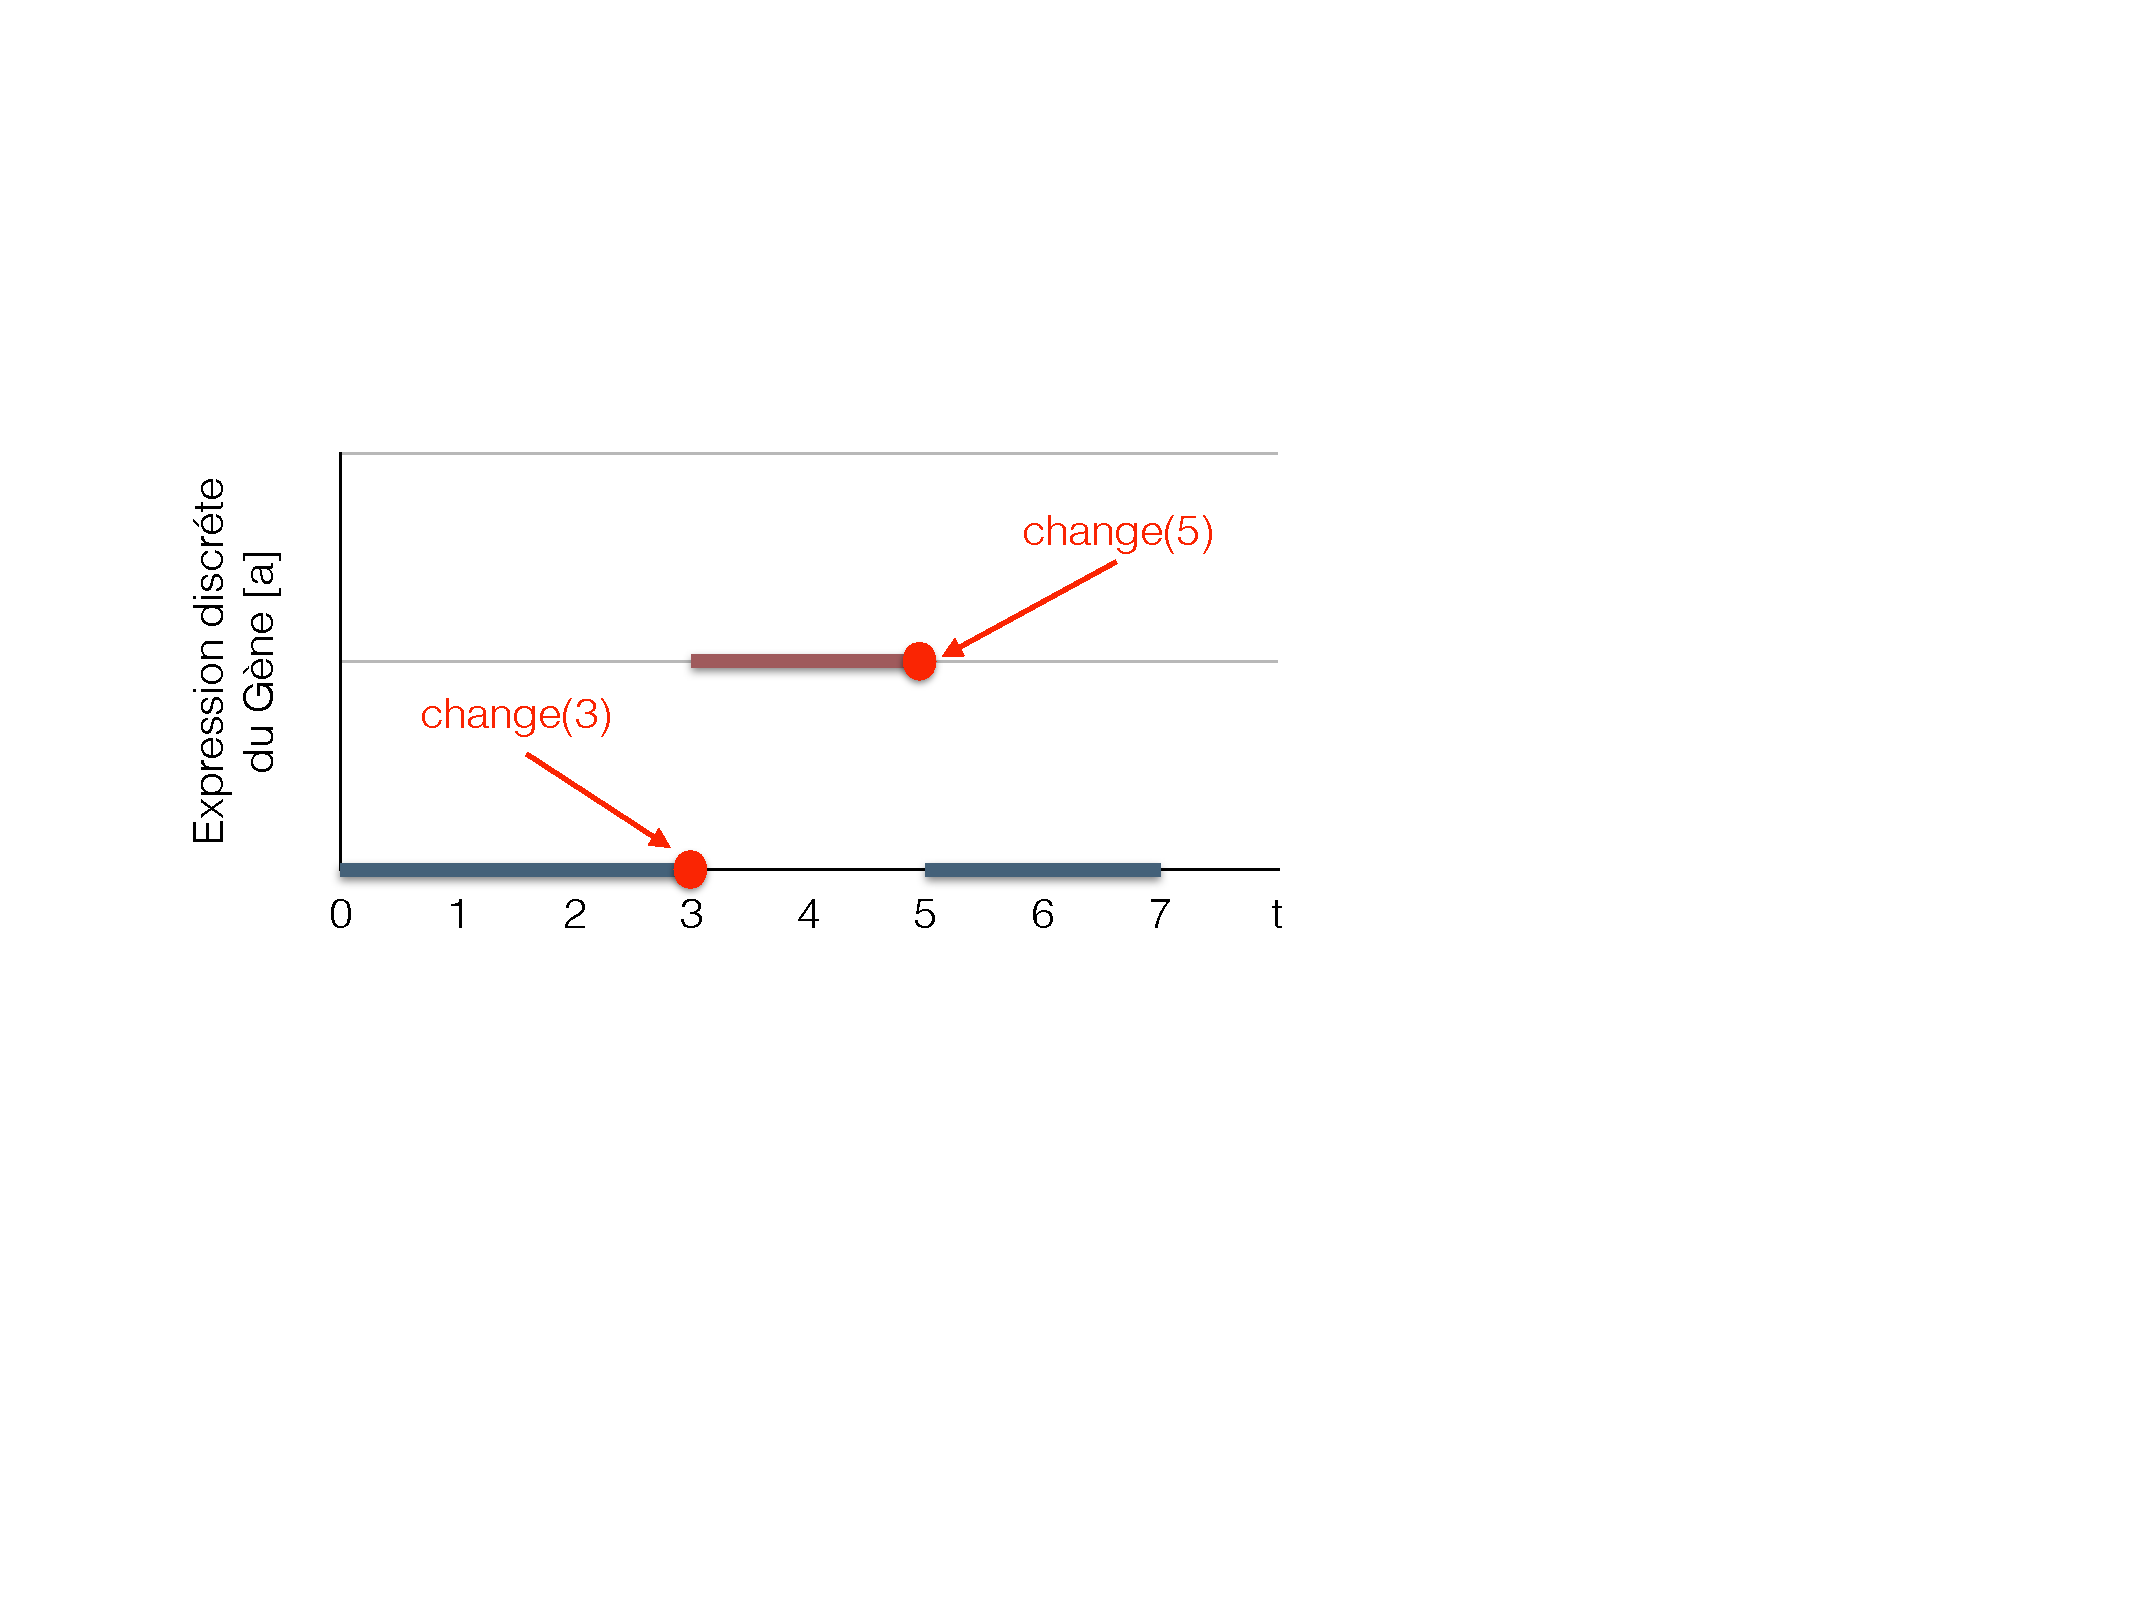
\includegraphics[width =0.31\linewidth]{images/courbes/gene-a-disc-change.pdf}
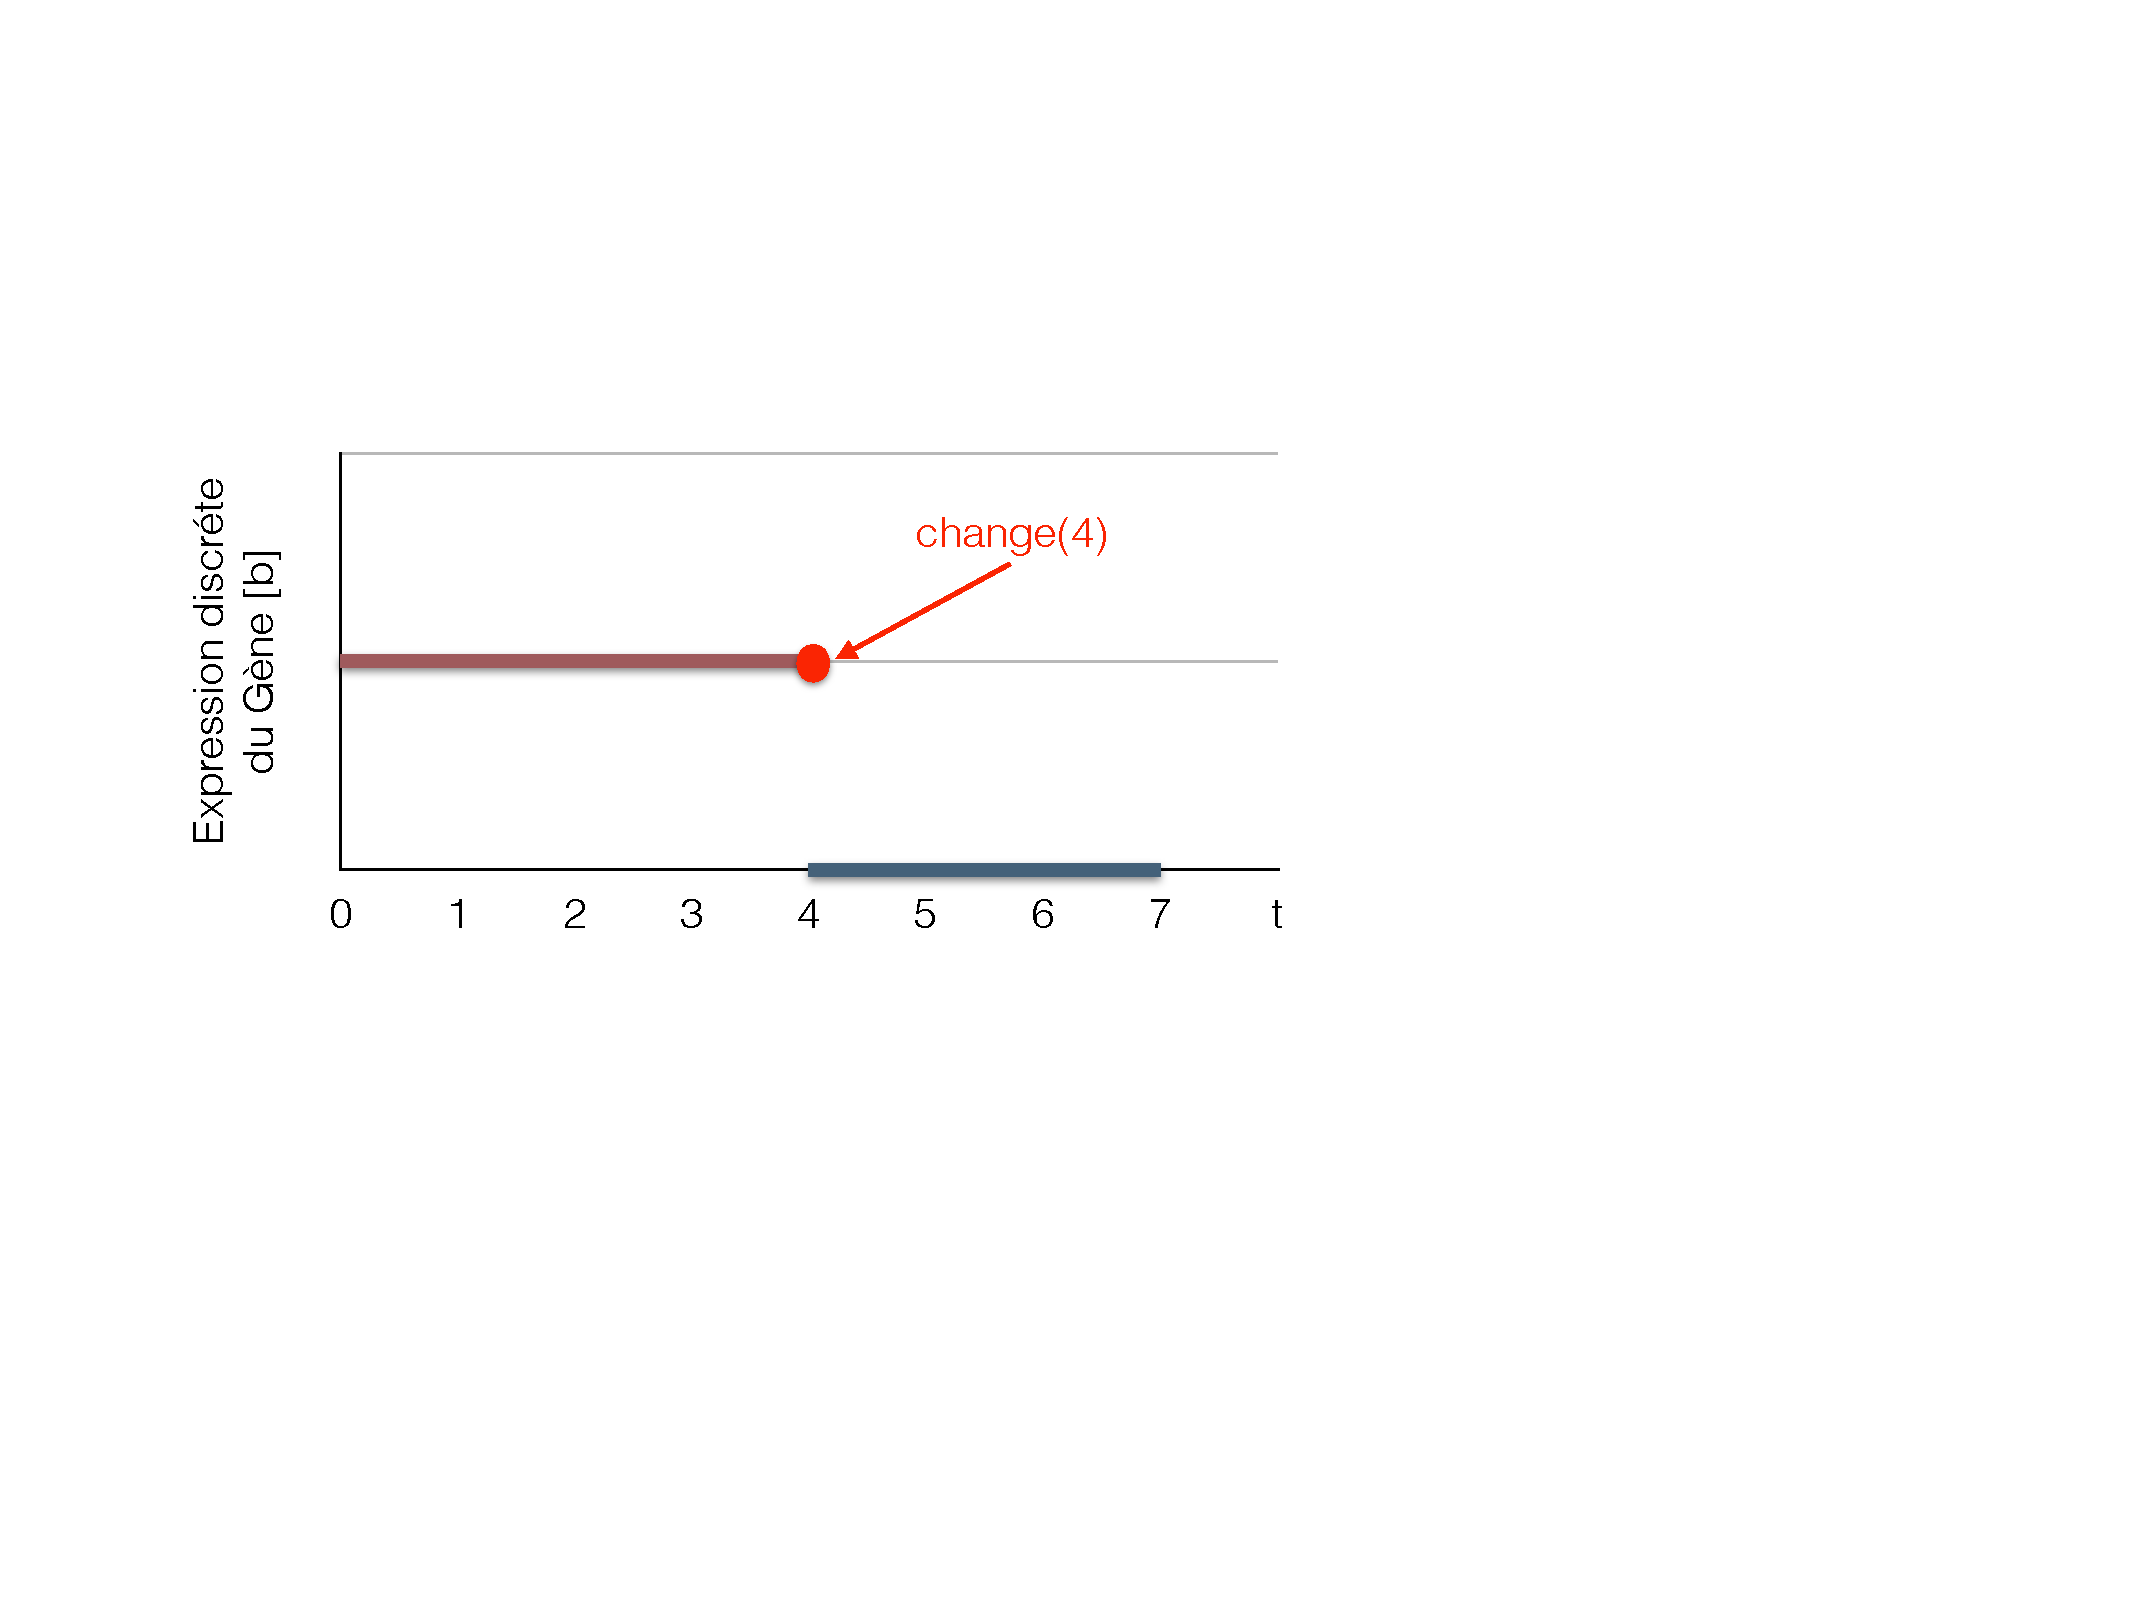
\includegraphics[width =0.31\linewidth]{images/courbes/gene-b-disc-change.pdf}
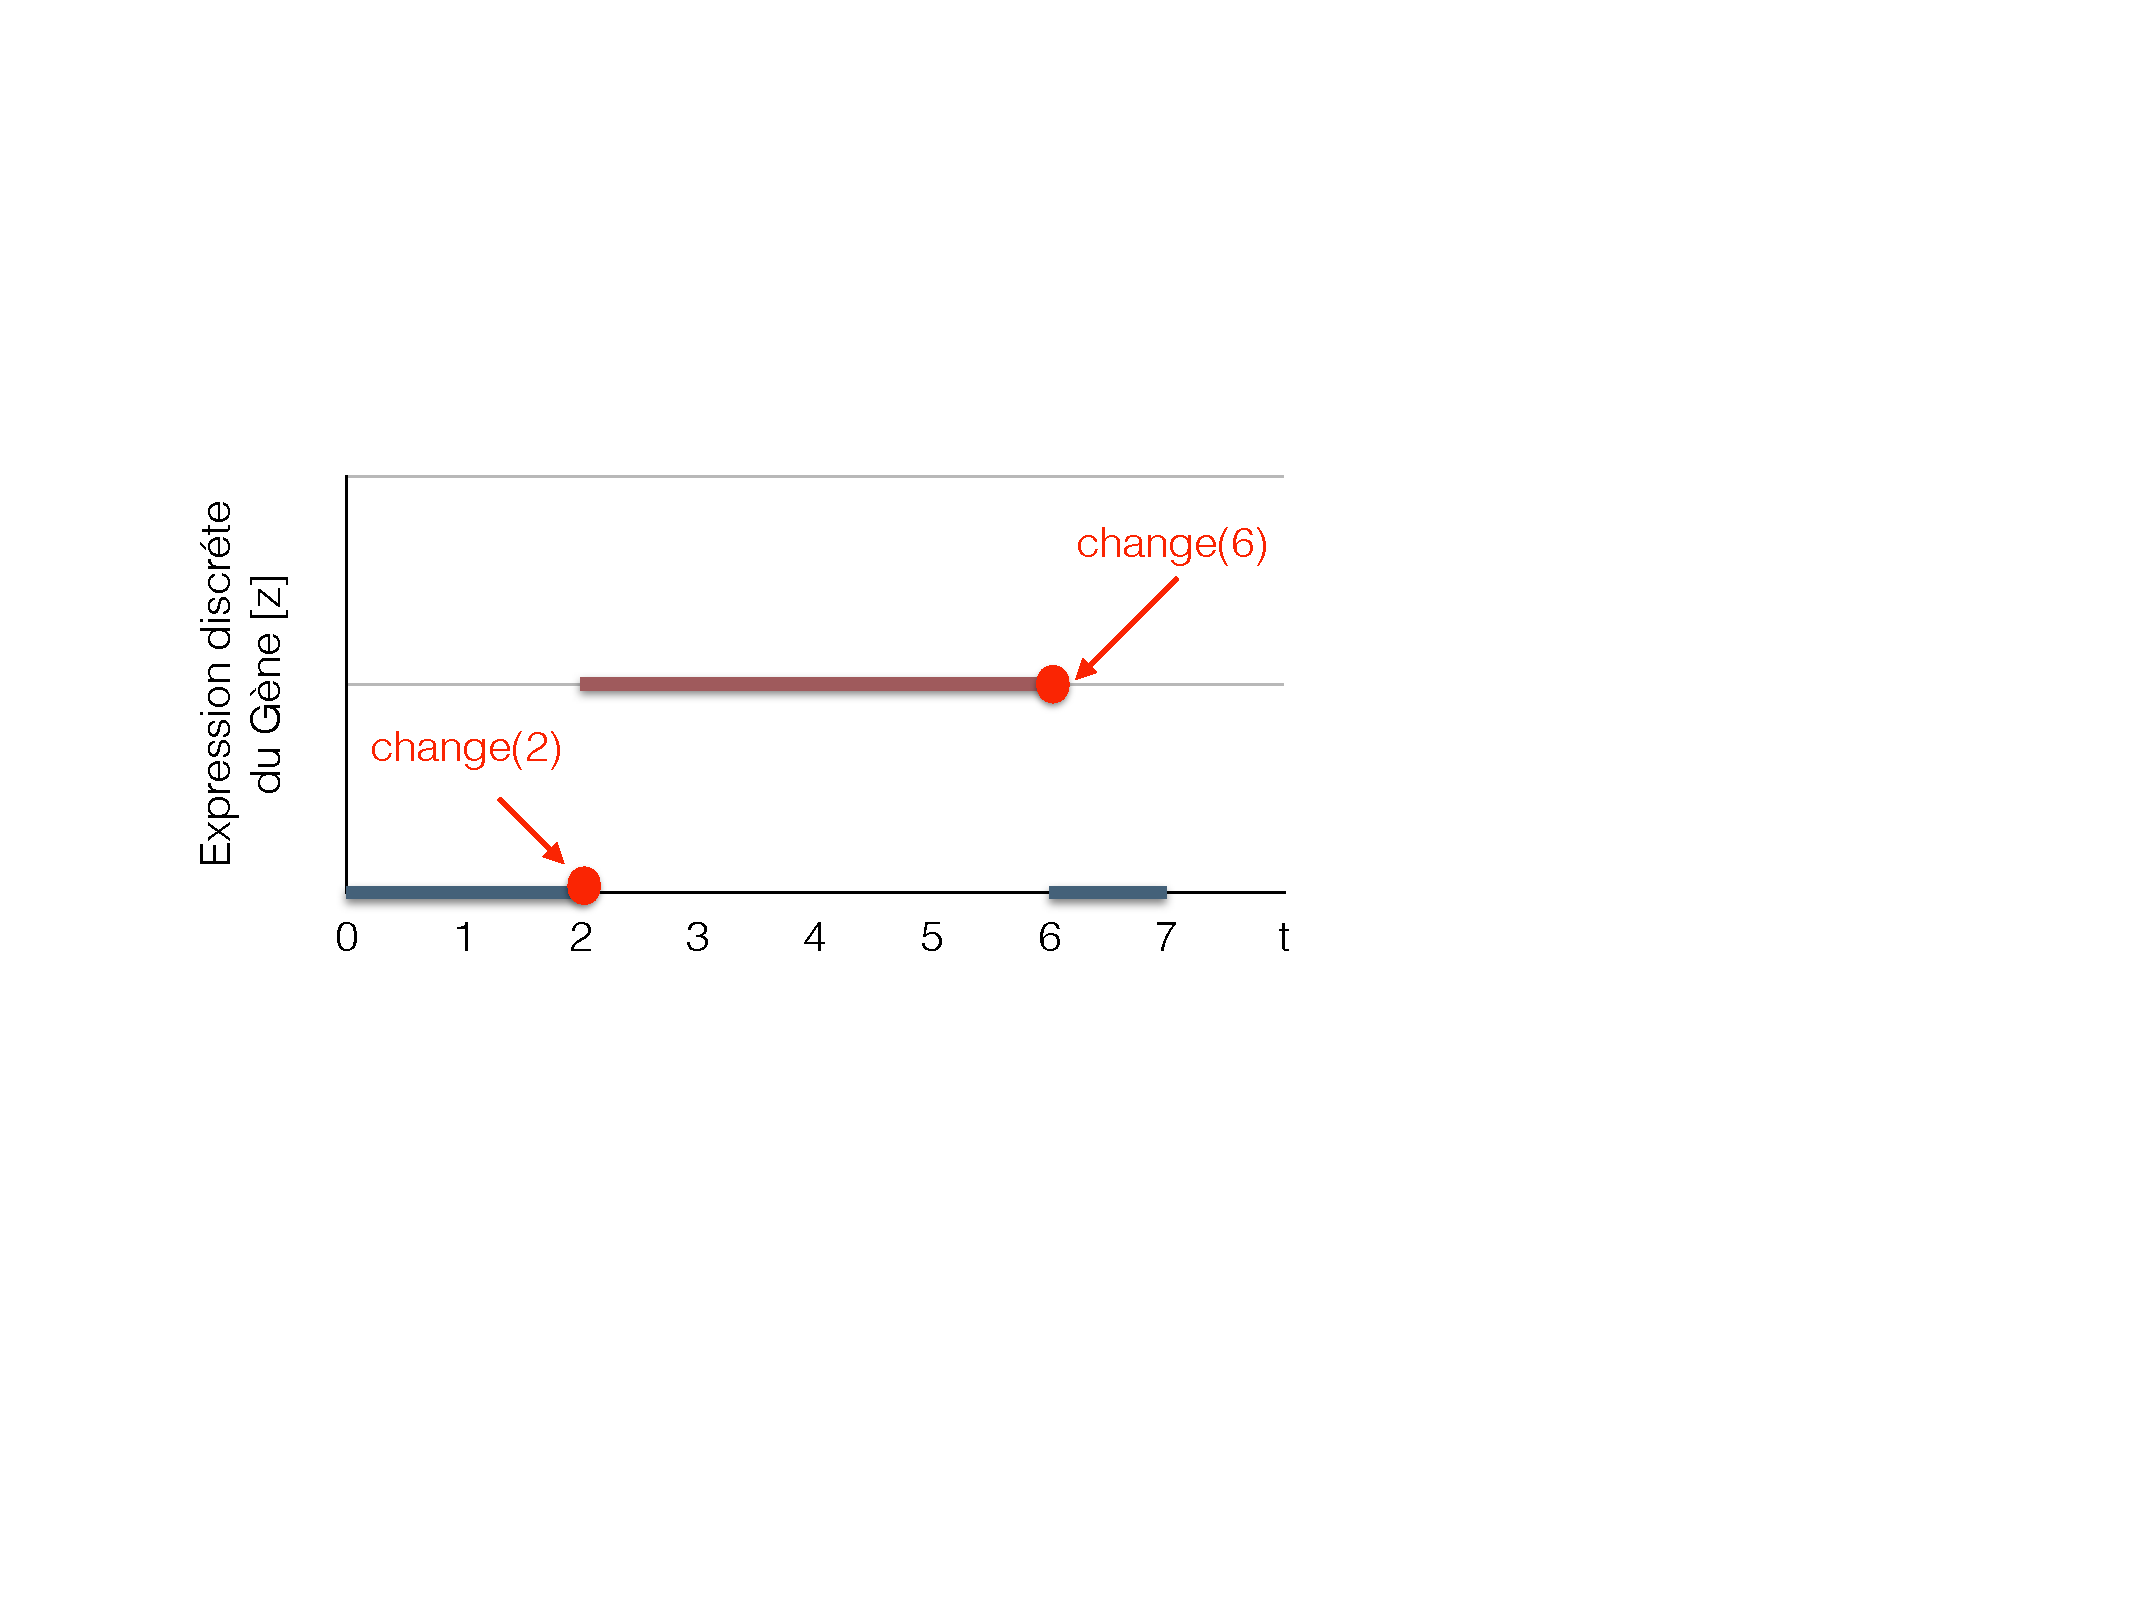
\includegraphics[width =0.31\linewidth]{images/courbes/gene-z-disc-change.pdf}
\caption{Examples of the discretization of continous time series data into bi-valued chronograms.
Abscisse represents time and ordinate the gene expression level.
The expression level is discretized according to a treshold fixed to the half of the gene expression value in this example. A \texttt{change(t)} is a time step in which we observe a change in the gene expression level. }
\label{fig:discretization}
\end{figure}

We can summarrize our method in the following steps:
\begin{itemize}
\item[-] Detection of changes
\item[-] Computation of the interactions possibly reponsible of thoses changes
\item[-] Filtering of the candidates actions
\item[-] Add actions to the model: generation/revision of the model
\end{itemize}

% Running example

We will now show an example of the execution of the Algorithm \pref{alg:PHG_ap} on the chronograms of the observed data of \pref{fig:discretization}:

%Let $i$ be the maximal number of hitters in an action of a PH: {\textit the indegree}.

The first change occurs at $t_1$ = $t_{min}$ = 2,
wich we will denote as \texttt{change(2)}. It is the gene \texttt{"z"} whose value changes from $0$ to $1$, thus the action that has realized this change is of the form $h = \PHfrappedelay{A}{D}{z_0}{z_1}$,
where $ A \in \PHl^{\diamond}, | A| \leq i$, (we suppose $i=2$) and $D$ is the delay wich is equal to $2$ here, since
$D_{t_i}=t_i - t_{i-1}$, such that $\exists$ \texttt{change($t_i$)} and \texttt{change($t_{i-1}$)},
$D_{t_1}= t_1 - t_0 = 2 - 0 = 2$.

Let $R=\{ b \rightarrow z, a \rightarrow z, a \rightarrow a \}$
be the set of regulation influences amoung the components of the system.
%
In the first change $t_1$ = 2 that we will denotes as $change(2)$,
It has been caused by an action $h = \PHfrappedelay{A}{2}{z_0}{z_1}$. According to $R$ the genes having influence \texttt{z} are $G_{R_z} = \{\texttt{a, b}\}$. It means that $A= \{ a_{\textcolor{red}{?}}, b_{\textcolor{red}{?}} \} $ or $A= \{ a_{\textcolor{red}{?}} \} $ or $A= \{ b_{\textcolor{red}{?}} \} $.
%
The expression level of the genes of $G{R_z}$ between $t_i$ and $t_{i-1}$ is computed from the observations as follows:
\begin{itemize}
\item[-] $a \in  G{R_z}$: $[a]_t=0$ $\forall t \in [0,2] $
\item[-] $b \in  G{R_z}$: $[b]_t=1$ $\forall t \in [0,2] $
\end{itemize}
%
Thus $A= \{ a_0, b_1 \} $ or $A= \{ a_0\} $ or $A= \{ b_1 \} $ and the set of candidate actions is:
$H_{change(2)} = \{ h_1=\PHfrappedelay{a_0}{2}{z_0}{z_1}
, h_2=\PHfrappedelay{b_1}{2}{z_0}{z_1}
, h_3=\PHfrappedelay{a_0 \wedge b_1 }{2}{z_0}{z_1} \}$.

The second change occurs at $t_2 = 3$ and we will denote it as $change(3)$.
Here its the gene \texttt{"a"} whose value changes from $a_0$ to $a_1$, thus the action that has realized this change is of the form
$h = \PHfrappedelay{A}{D}{a_0}{a_1}$ 
where $ A \in \PHl^{\diamond}, | A| \leq 2$ and $D$ is the delay that is equal to $1$ here: 
$D_{t_2}= t_2 - t_1 = 3 - 2= 1$.
According to $R$ the genes which influence \texttt{"a"} are $G_{R_a} = \{\texttt{a}\}$.
It means that $A= \{ a_{\textcolor{red}{?}}\}$ and the expression level of \texttt{"a"} between $t_1$ and $t_{2}$ is $a_0$.
So  $A= \{ a_0\} $ and it is an auto-influence. Thus there is only one candidate action that is a \emph{self-action}:
$H_{change(3)} = \{ h=\PHfrappedelay{a_0}{1}{a_0}{a_1}  \}$.

The third change occurs at $t_3 = 4$ and we will denote it as $change(4)$.
Here it is the gene \texttt{"b"} whose value changes from $b_1$ to $b_0$, thus the action that has realized this change is of the form 
$h = \PHfrappedelay{A}{D}{b_1}{b_0}$ where $ A \in \PHl^{\diamond}, | A| \leq 2$ and $D$ is the delay and it is equal to $1$ ($D_{t_3}= t_3 - t_2 = 4 - 3 = 1$).
According to $R$ there is no gene that can influences \texttt{"b"}, thus no action can realizes this change.

The fourth change occurs at $t_4 = 5$ and we will denote it as $change(5)$.
Here it is \texttt{"a"} whose value changes from $a_1$ to $a_0$, thus the action that has realized this change is of the form $h = \PHfrappedelay{A}{D}{a_1}{a_0}$ \\
where $ A \in \PHl^{\diamond}, | A| \leq 2$ and $D$ is the delay that is equal to $1$ ($D_{t_4}= t_4 - t_3 = 5 - 4= 1$).
According to $R$ the genes which influence \texttt{"a"} are $G_{R_a} = \{\texttt{a}\}$.
Again $A= \{ a_{\textcolor{red}{?}}\}$ and since the expression level of \texttt{a} between $t_3$ and $t_{4}$ is $a_1$,
we have $A= \{ a_1\} $ and there is only one candidate action that is a \emph{self-action}
$H_{change(5)} = \{ h=\PHfrappedelay{a_1}{1}{a_1}{a_0} \}$.

The fifth change occurs at $t_5 = 6$ and we will denote it as $change(6)$.
Here it is \texttt{"z"} whose value changes from $z_1$ to $z_0$, thus the action that has realized this change has the form of:
$h = \PHfrappedelay{A}{D}{z_1}{z_0}$ \\
where $ A \in \PHl^{\diamond}, |A| \leq 2$ and $D$ is equal to 1 here:
$D_{t_5}= t_5 - t_4 = 6 - 5= 1$ \\
According to $R$, $G_{R_z} = \{\texttt{a, b}\}$.
It means that $A= \{ a_{\textcolor{red}{?}}, b_{\textcolor{red}{?}} \} $ or $A= \{ a_{\textcolor{red}{?}} \} $ or $A= \{ b_{\textcolor{red}{?}} \} $
The expression level of \texttt{"a"} and \texttt{"b"} between $t_4$ and $t_{5}$ is respectively $a_0$ and $b_0$.
Thus $A= \{ a_0, b_1 \} $ or $A= \{ a_0\} $ or $A= \{ b_0 \} $ \\
The candidates action are:
$H_{change(6)} = \{ h_1=\PHfrappedelay{a_0}{1}{z_1}{z_0}$, $  h_2=\PHfrappedelay{b_0}{1}{z_1}{z_0}$, $  h_3=\PHfrappedelay{a_0 \wedge b_0 }{1}{z_1}{z_0} \}$.

After proccessing all chronograms, the candidate actions are: \\
$H_{change(2)} = \{ h_1=\PHfrappedelay{a_0}{2}{z_0}{z_1},  h_2=\PHfrappedelay{b_1}{2}{z_0}{z_1}, h_3=\PHfrappedelay{a_0 \wedge b_1 }{2}{z_0}{z_1} \}$.\\
$H_{change(3)} = \{ h_4=\PHfrappedelay{a_0}{1}{a_0}{a_1}  \}$. \\
$H_{change(5)} = \{ h_5=\PHfrappedelay{a_1}{1}{a_1}{a_0}  \}$. \\
$H_{change(6)} = \{ h_6=\PHfrappedelay{a_0}{1}{z_1}{z_0}$ , $  h_7=\PHfrappedelay{b_0}{1}{z_1}{z_0}, h_8=\PHfrappedelay{a_0 \wedge b_0 }{1}{z_1}{z_0} \}$. \\

At this stage of the process, all canditates actions are consistent with all observations and given regulation influences.
Until now the method used ensured completeness: here we have the complete set of consistent action that can explain the observations.


